\section{Main results}


\subsection{Sample size imbalance}\label{sec_sizeratio}

 In this subsection, we consider the setting where $X^{(1)}$ and $X^{(2)}$ are independent and have the same population covariance matrices $\Sigma^{(1)}=\Sigma^{(2)}$. However, the two tasks can have different sample sizes $n_1\ne n_2$. In this case, we can obtain the exact asymptotic limits of the bias term \eqref{Lbias} and the variance term \eqref{Lvar}. We will use these results to illustrate the effects of the bias-variance tradeoff and varying sample sizes on the performance of the $\MTL$ estimator.

\begin{theorem}\label{cor_MTL_loss}
Under Assumption \ref{assm_big1}, suppose that $\Sigma^{(1)}=\Sigma^{(2)}$ and the entries of $Z^{(1)}$ and $Z^{(2)}$ are i.i.d. Gaussian random variables. Then for any small constant $\e>0$ and large constant $C>0$, there exists a high probability event $\Xi$, on which the following estimates hold uniformly in all $a\in \R$:
\be\label{Lvar_samplesize}
L_{\var}(a)= \sigma^2  \left[ \cal L_1(a)+ \OO\left({p^{c}}/{n_1}\right)\right]  ,
\ee
and
\begin{align}
L_{\bias}(a)&= \left[ \cal L_2(a)+  \OO\left(p^{-1/2+c}\right)\right] \cdot  \|\beta^{(1)}-a\beta^{(2)}\|^2 \nonumber\\
&+ \OO \left[ p^{-C}\left( \|\beta^{(1)} \|^2  +  \|\beta^{(2)} \|^2\right)   \right].\label{Lbias_samplesize}
	%-\left[1- \left( 1-\frac{1}{\sqrt{\rho_1}}\right)^4\right] pd^2\cdot \frac{\rho_1^2 (\rho_1+\rho_2)}{(\rho_1 + \rho_2 - 1)^3} +\OO(p^{-c}\sigma^2)  \le
	%   \left|L(\hat{\beta}_2^{\MTL}) - \frac{2d^2 n_1^2 (n_1 + n_2)}{(n_1 + n_2 - p)^3} -\frac{\sigma^2 p}{n_1 + n_2 - p}  \right|
	% \le \varepsilon \cdot \frac{2d^2 n_1^2 (n_1 + n_2)}{(n_1 + n_2 - p)^3} +  \OO(p^{-c/2}).\label{cor_MTL_error}
	%\left[\left( 1+\frac{1}{\sqrt{\rho_1}}\right)^4-1\right] d^2\cdot \frac{\rho_1^2 (\rho_1+\rho_2)}{(\rho_1 + \rho_2 - 1)^3} \\
	%& +C \left[(p^{-c_\varphi}+p^{-c_\infty/2})(\sigma^2 +d^2)+p^{-c_\infty}\kappa^2 + %\frac{d^4+\sigma^2 d^2}{\kappa^2}\right],\nonumber
	 \end{align}
Here we define the functions
\begin{align*}
&\cal L_1(a):= \frac{2p}{  {n_2} (1-\xi_2) + a^2 n_1 (1-\xi_1)+ \sqrt{[ {n_2} (1-\xi_2) +a^2 n_1 (1-\xi_1)]^2 + 4a^2{n_2}{n_1} (\xi_1+\xi_2 -\xi_1\xi_2)}}, \\
&\cal L_2(a): = \frac1{a^2}\cdot \frac{1- 2\frac{\cal L_1(a)}{\xi_2[1 + \cal L_1(a)]} + \kappa(a)}{1- \xi_2 \kappa(a)},
\end{align*}
where we abbreviate $\xi_1:=p/n_1$, $\xi_2:=p/n_2$ and
\begin{align*}
\kappa(a):= \frac{\cal L_1(a)^2}{\xi_2^2[1+\cal L_1(a)]^2}  \left[1 - \frac{a^4 \cal L_1(a)^2 }{\xi_1[1+a^2\cal L_1(a) ]^2}\right]^{-1}.
%f_2(a):= \frac{a^4 \cal L_1(a)^2}{\xi_1^2 } \left[1 - \frac{a^4 \cal L_1(a)^2 }{\xi_1[1+a^2\cal L_1(a) ]^2}\right]^{-1},\\
%f_3(a):= \frac1{a^2}\frac{\xi_1}{\xi_2 +\cal L_1(a)}
 \end{align*}
%	In the setting of Example \ref{ex_sample_ratio}, assume that
%	%a) the sample sizes $n_1$ and $n_2$ are greater than $(1 + \tau) p$, b) $\Sigma_1=\Sigma_2=\id_p$, and c) %there exists a small constant $c_0>0$ such that
%	(i) both tasks sample sizes are at least $3p$;
%	(ii) noise variance is smaller than the shared signal variance: $\sigma^2 \lesssim  \kappa^2$;
%%	\be\label{choiceofpara0}
%%	p^{-1/2+c_0}\sigma^2 + p^{c_0}d^2\le \kappa^2\le p^{1-c_0} (\sigma^2 +d^2)  .  	\ee
%	%\be\label{choiceofpara0}
%%	(ii) the task-specific variance of $\beta_i$ is much smaller than the signal strength {\color{red}$d^2 = \oo( {\kappa^2})$}; \HZ{what does $\ll$ mean exactly?}
%%	(iii) the sample sizes $n_1$ and $n_2$ are greater than $(1 + \tau) p$.
%	(iii) task-specific variance is much smaller than the shared signal variance: $d^2 \le p^{-\e}{\kappa^2}$ for a small constant $c>0$.
%	Let $\varepsilon = (1 + \sqrt{p/n_1})^ 4 - 1$, which decreases as $n_1$ increases.
%	Let $\hat{A},\hat{B}$ be the global minimizer of $f(A, B)$.
%	With high probability over the randomness of the input,
%	the prediction loss of $\hat{\beta}_2^{\MTL} = \hat{B} \hat{A}_2$ for task two satisfies that
%	\begin{align}
%	%-\left[1- \left( 1-\frac{1}{\sqrt{\rho_1}}\right)^4\right] pd^2\cdot \frac{\rho_1^2 (\rho_1+\rho_2)}{(\rho_1 + \rho_2 - 1)^3} +\OO(p^{-c}\sigma^2)  \le
%	   \left|L(\hat{\beta}_2^{\MTL}) - \frac{2d^2 n_1^2 (n_1 + n_2)}{(n_1 + n_2 - p)^3} -\frac{\sigma^2 p}{n_1 + n_2 - p}  \right|
%	\le \varepsilon \cdot \frac{2d^2 n_1^2 (n_1 + n_2)}{(n_1 + n_2 - p)^3} +  \OO(p^{-c/2}).\label{cor_MTL_error}
%	%\left[\left( 1+\frac{1}{\sqrt{\rho_1}}\right)^4-1\right] d^2\cdot \frac{\rho_1^2 (\rho_1+\rho_2)}{(\rho_1 + \rho_2 - 1)^3} \\
%	%& +C \left[(p^{-c_\varphi}+p^{-c_\infty/2})(\sigma^2 +d^2)+p^{-c_\infty}\kappa^2 + %\frac{d^4+\sigma^2 d^2}{\kappa^2}\right],\nonumber
%	 \end{align}
%	 with high probability for any fixed $c\in(0, \min(\frac{1}{4}, \delta,\frac{\varphi-4}{2\varphi}))$.
%	 {\color{red}[FY: the error also contains $p^{-1/2+2c}\kappa^2 +  p^{-1/4+c} (\sigma^2 +d^2) $, both of which cannot be omitted, because (i) there is no assumption on the upper bound of $\kappa^2$, and (ii) we do not necessarily have $c_\varphi<1/4$. We can decide how to present the result concisely (for instance we can impose an upper bound on $\kappa^2$ and that $c_\varphi<1/4$), but it needs to be correct.]}
	 \end{theorem}

\iffalse
 We need to state a result for Gaussian matrix ...... Consider
$$f (\al,n_1,n_2)= \frac1p\tr\left[\frac{1}{ (X_1^\top X_1 + \al \cdot X_2^\top X_2)^2} (X_1^\top X_1)^2\right].$$
In our case, we have $\al=1$, but we can handle more general $\al$. We introduce two parameters:
$$a= \al \frac{n_2}{n_1} \left( \frac{p}{n_1} + \frac{p}{n_2}- \frac{p}{n_1 }\cdot \frac{p}{n_2}\right),\quad b= \al \frac{n_2}{n_1}\left( 1- \frac{p}{n_2}\right) + \left( 1- \frac{p}{n_1}\right). $$
Then we define the following parameters:
\begin{align*}
x= \frac{-b+ \sqrt{b^2 + 4a}}{2a},\quad y= \left[ x^{-2} - \frac{p}{n_1}\left( 1+\frac{p}{n_1}x\right)^{-2}\right]^{-1},\quad \omega= \al\frac{n_2}{n_1} \left( 1 + \al \frac{p}{n_1}x\right)^{-1}.
\end{align*}
We have that
$$f(\al,n_1,n_2)= \frac{1 - 2\omega x + \omega^2 y}{ 1 - \frac{p}{n_2} \cdot \omega^2 y } +\oo(1)\quad \text{w.h.p.} $$
In the setting $\al=1$, both $\omega x$ and $\omega^2 y$ can be written in terms of only one parameter
%$$f(\al,n_1,n_2)= \frac{\left(u^2 -\frac{p}{n_1}\right) \left(1- 2\frac{n_2}{n_1}  u^{-1}\right) + \frac{n_2^2}{n_1^2} }{ u^2 -\frac{p}{n_1}\left(1 + \frac{n_2}{n_1}\right) } +\oo(1)\quad \text{w.h.p.} $$
%where
$$u: = x^{-1}\left(1+\frac{p}{n_1}x\right)=   \frac{ b+\sqrt{b^2+4a}}{2} +\frac{p}{n_1}   .$$
\fi

We believe the convergence rates $p^c/n_1$ and $p^{-1/2+c}$ in \eqref{Lvar_samplesize} and \eqref{Lbias_samplesize} are both sharp up to the $p^c$ factor. The proof of Theorem \ref{cor_MTL_loss} will be given in Appendix \ref{app_iso_cov} in the supplement \cite{MTL_suppl}. For the variance estimate in \eqref{Lvar_samplesize}, it is not necessary to assume the Gaussian distributions of the $Z^{(1)}$ and $Z^{(2)}$ entries. In fact, \eqref{Lvar_samplesize} is a special case of Theorem \ref{thm_main_RMT} below for the more general case with possibly different $\Sigma^{(1)}$ and $\Sigma^{(2)}$. On the other hand, the Gaussian assumption is needed in our current proof of the bias limit \eqref{Lbias_samplesize}. In the setting of Theorem \ref{cor_MTL_loss}, we can write
\begin{align*}
L_{\bias} (a)&=\bv_a^\top (Z^{(1)})^\top Z^{(1)} \frac1{ \left[a^2(Z^{(1)})^\top Z^{(1)}+ (Z^{(2)})^\top Z^{(2)}  \right]^{2}}(Z^{(1)})^\top Z^{(1)} \bv_a,
\end{align*}
where we abbreviate $\bv(a):=(\Sigma^{(1)})^{1/2}\left(a\beta^{(1)}- a^2\beta^{(2)}\right)$. By the rotational invariance of $(Z^{(1)})^\top Z^{(1)}$ and $(Z^{(2)})^\top Z^{(2)}$, we have that
\begin{align}\label{Lbias_idea}
L_{\bias} (a)&\approx \|\bv_a\|^2 \frac1p\bigtr{ [(Z^{(1)})^\top Z^{(1)}]^2 \frac1{ \left[a^2(Z^{(1)})^\top Z^{(1)}+ (Z^{(2)})^\top Z^{(2)}\right]^{2}}  },
\end{align}
up to a small error. Notice that we can write \eqref{Lbias_idea} into a simpler form
\begin{align}\nonumber %\label{Lbias_idea2}
L_{\bias} (a)&\approx \|\bv_a\|^2 \left. \frac{\dd }{\dd x}\right|_{x=0}\frac1p\bigtr{  \frac1{ a^2(Z^{(1)})^\top Z^{(1)}+ x[(Z^{(1)})^\top Z^{(1)}]^2+(Z^{(2)})^\top Z^{(2)} }  }.
\end{align}
It is well-known that the empirical spectral distributions (ESD) of $(Z^{(i)})^\top Z^{(i)}$, $i=1,2$, satisfy the famous Marchenko-Pastur (MP) law asymptotically \cite{MP}. From the MP law of $(Z^{(1)})^\top Z^{(1)}$, we can also derive the asymptotic ESD of $a^2(Z^{(1)})^\top Z^{(1)}+ x[(Z^{(1)})^\top Z^{(1)}]^2$ for any fixed $a\in \R$ and $x>0$. Due to the rotational invariance of multivariate Gaussian distributions,
%$a^2(Z^{(1)})^\top Z^{(1)}+ x[(Z^{(1)})^\top Z^{(1)}]^2$ and $(Z^{(2)})^\top Z^{(2)}$ are asymptotically freely independent from each other \cite{nica2006lectures}. Hence
the asymptotic ESD of $a^2(Z^{(1)})^\top Z^{(1)}+ x[(Z^{(1)})^\top Z^{(1)}]^2+(Z^{(2)})^\top Z^{(2)}$ is given by the free additive convolution (or free addition) of the asymptotic ESD of $a^2(Z^{(1)})^\top Z^{(1)}+ x[(Z^{(1)})^\top Z^{(1)}]^2$ and the MP law of $(Z^{(2)})^\top Z^{(2)}$\cite{nica2006lectures}. In particular, a sharp convergence estimate has been proved in \cite{BES_free1,BES_free2} for the free addition of two probability measures. We use that result to obtain a convergence estimate on
$$\frac1p\bigtr{  \frac1{ a^2(Z^{(1)})^\top Z^{(1)}+ x[(Z^{(1)})^\top Z^{(1)}]^2+(Z^{(2)})^\top Z^{(2)} }  }.$$
Taking derivative with respect to $x$ at $x=0$ gives the exact asymptotic limit of $L_{\bias}(a)$. We refer the reader to Appendix \ref{app_iso_cov} of the supplement \cite{MTL_suppl} for more details.

We believe that the above argument can be extended to the case without the Gaussian assumption. For example, instead of using the results in \cite{BES_free1,BES_free2} on free addition, we can use the sharp local laws on polynomials of random matrices in \cite{EKN_poly}. However, to apply the result in \cite{EKN_poly}, we need to check some difficult technical regularity conditions for our setting, which is not the focus of this work. Hence we do not pursue this direction in this paper.


\paragraph{Examples.}
First, we show that if $\|\beta_0\|^2 \gg d^2$, then the global minimizer $\hat a$ of the function $g(a)$ in \eqref{eq_mtl_A12} is close to $1$.
	The proof of Proposition \ref{lem_hat_v} will be given in Appendix \ref{app_iso_cov_prop}.

	\begin{proposition}\label{lem_hat_v}
%Suppose the assumptions of Lemma \ref{prop_model_shift_tight} hold. Assume that $ \kappa^2 \sim pd^2 \sim \sigma^2$ are of the same order.
Suppose Assumption \ref{assm_big1} and the above setting of random effect model hold. %in Example \ref{ex_same_cov} hold.
Suppose that for a constant $c_0>0$,
	\be\label{para_rel}
	 \|\beta_0\|^2 \ge p^{c_0}d^2 +p^{-1/2+c_0}\sigma^2.
	\ee
 Then we have that for any small constant $c>0$ and large constant $ C>0$,
	%Let $c$ be a sufficiently small fixed constant.
	%In the setting of Corollary \ref{cor_MTL_loss},
%There exists a constant $C>0$ such that
	\be\label{hatw_add1}
	 \hat a =1+ \OO\left(\frac{d^2}{\|\beta_0\|^2} + p^{-1/4+c} \frac{d+\sigma}{\|\beta_0\|} + p^{-C}\right) \quad \text{w.h.p.}
	\ee
\end{proposition}
%Suppose every $\beta^{(i)}$ consists of two random components, one that is shared among all tasks and one that is task-specific.
%%Thus, each task contributes a certain amount to the shared component and injects a task-specific bias.
%More precisely, %we have
%$$\beta^{(i)}=\beta_0 +\wt \beta^{(i)},\quad i=1,2,\cdots, t,$$
%where $\beta_0$ denotes the shared component, %whose entries are i.i.d. Gaussian random variables of mean zero and variance $p^{-1}\kappa^2$,
%and $\wt \beta^{(i)}$ denotes the $i$-th
%%Let $\beta^{(i)}$ be equal to $\beta_0$ plus a
%task-specific component whose entries are i.i.d. Gaussian random variables of mean zero and variance $p^{-1} d^2$.

We emphasize that unlike Theorem \ref{cor_MTL_loss}, for Proposition \ref{lem_hat_v} we do not assume $\Sigma^{(1)}=\Sigma^{(2)}$ and the Gaussian distributions of the entries of $Z^{(1)}$ and $Z^{(2)}$. Combining Lemma \ref{lem_HPS_loss}, Theorem \ref{cor_MTL_loss} and Proposition \ref{lem_hat_v}, and using  that $\|\beta^{(1)}-\beta^{(2)}\|^2 = (2+\oo(1))d^2$ with high probability, the predication loss $L(\hat{\beta}_2^{\MTL}(\hat a)) $ is approximately equal to
$$\ell(n_1,n_2)= \sigma^2 \cal L_1(1) +   2d^2 \cal L_2(1)= \frac{p\sigma^2}{n_1+n_2-p} +  2d^2  \frac{n_1^2 (n_1+n_2-p)+p n_1n_2}{(n_1+n_2)^2(n_1+n_2-p)}, $$
with high probability, where in the second step we obtain $\cal L_1(1)$ and $\cal L_2(1)$ through direct calculations.
Now we compare $\ell(n_1,n_2)$ with \eqref{L_STL_simple01}. First, we notice that the variance term $\sigma^2 \cal L_1(1)$ is smaller than $L(\hat{\beta}_2^{\STL} )$, while the bias term always increases (because the bias in single-task linear regression is zero). This gives a \emph{bias-variance tradeoff} for the predication loss of the HPS estimator. Second, calculating the derivative with respect to $n_1$, it is not hard to see that the variance term always decreases as $n_1$ increases, while the bias term always increases with $n_1$. Hence how the performance of the HPS estimator changes with respect to $n_1$ also depends on an intricate bias-variance tradeoff.

Now fix an $n_2$, we study the bias-variance tradeoff with respect to $n_1$ using the following function of $\rho:=\rho_1+\rho_2$, which is $L(\hat{\beta}_2^{\STL} )-\ell(n_1,n_2)$ divided by $2d^2$:
$$h(\rho):=\frac{p }{n_2-p}\cdot \frac{\sigma^2}{2d^2}- \frac{\ell(\rho_1p , \rho_2p)}{2d^2}  = \frac{\rho-\rho_2}{(\rho-1)(\rho_2-1)}\cdot \frac{\sigma^2}{2d^2}- \frac{(\rho-\rho_2)^2 (\rho-1)+(\rho-\rho_2)\rho_2}{\rho^2(\rho-1)}  .$$
This function characterizes $L(\hat{\beta}_2^{\STL} )-L(\hat{\beta}_2^{\MTL}(\hat a)) $, and hence gives the quantitive information transfer from the source task to the target task.
First, we have positive (resp. negative) transfer if and only if $h(\rho)>0$ (resp. $h(\rho)<0$). Moreover, the sign of $h(\rho)$ is determined by the sign of the second order polynomial %which is equivalent to the following inequality:
\be\label{poly1} \left( \frac{1}{\rho_2-1}\cdot \frac{\sigma^2}{2d^2}-1 \right)\rho^2 + ( \rho_2+1)\rho - 2\rho_2 .\ee
We observe the following dichotomy. %\FY{add several plots to illustrate this dichotomy}
\begin{enumerate}
\item If $\frac{1}{\rho_2-1}\cdot \frac{\sigma^2}{2d^2}-1 >0$, then the polynomial \eqref{poly1} is positive for all $\rho\in (\rho_2+1,\infty)$, so that the transfer is always positive.

\item If $\frac{1}{\rho_2-1}\cdot \frac{\sigma^2}{2d^2}-1 < 0$, then we have the following cases.

\begin{itemize}
\item If $(\rho_2+1)^2 < 8\rho_2 \left( 1- \frac{1}{\rho_2-1}\cdot \frac{\sigma^2}{2d^2}  \right)$, the polynomial \eqref{poly1} is negative for all $\rho$, so that the transfer is always negative.

\item If $(\rho_2+1)^2 > 8\rho_2 \left( 1- \frac{1}{\rho_2-1}\cdot \frac{\sigma^2}{2d^2}  \right)$, the polynomial \eqref{poly1} has two positive roots, where one of them is always smaller than $\rho_2+1$. Hence if the larger root, say $\rho_c$, is smaller than $\rho_2+1$, then the transfer is always negative for $\rho\in (\rho_2+1,\infty)$; otherwise, there is a transition from positive transfer to negative transfer as $\rho$ crosses $\rho_c$.
\end{itemize}
\end{enumerate}
Second, we calculate the derivative of $h(\rho)$, and find that its sign  is determined by the sign of the third order polynomial
\be\label{poly2}
 \frac{1}{\rho_2}\cdot \frac{\sigma^2}{2d^2} \rho^3 - 2(\rho-\rho_2)(\rho-1)(\rho-2)   - (\rho_2-1)\rho .\ee
Then we observe the following dichotomy. %\FY{add several plots to illustrate this dichotomy}
\begin{enumerate}
\item If $\frac{1}{\rho_2}\cdot \frac{\sigma^2}{2d^2} > 2$, the polynomial \eqref{poly2} is always positive for all $\rho\in (\rho_2+1,\infty)$, so that the information transfer always increases as $n_1$ increases.

\item If $\frac{1}{\rho_2}\cdot \frac{\sigma^2}{2d^2} < 2$, the polynomial \eqref{poly2} is positive initially around $\rho=\rho_2+1$, and then becomes negative when $\rho$ crosses its unique root, say $\rho_c$, in $(\rho_2+1,\infty)$. Hence the information transfer achieves the global maximum at $\rho=\rho_c$.
\end{enumerate}

%where $w_0:={\sigma^2}/{2d^2}$ is the ratio between the model bias and the noise variance.
%and $$ h_1(\rho_1,\rho_2):= \frac{\rho_1}{(\rho_1+\rho_2-1)(\rho_2-1)},\quad h_2(\rho_1,\rho_2):= \frac{\rho_1^2 (\rho_1+\rho_2-1)+\rho_1\rho_2}{(\rho_1+\rho_2)^2(\rho_1+\rho_2-1)}.$$
\iffalse
Then whether $L(\hat{\beta}_2^{\MTL}(\hat a)) $ is larger or smaller than

Applying Theorem \ref{thm_main_RMT} to the above setting, we get that
	\begin{align*}
		\frac{1}{n_1 + n_2} \tr[\Sigma^{(2)} (a_1\Sigma^{(1)} + a_2\Sigma^{(2)})^{-1}]
		= \frac{1}{n_1 + n_2} \bigtr{((a_1 + a_2)\id_p)^{-1}}
		= \frac{p}{n_1 + n_2 - p},
	\end{align*}
	because $a_1 + a_2 = 1 - \frac{p}{n_1 + n_2}$ by equation \eqref{eq_a12extra}.
	%Similarly, for the bias limit, we solve the self-consistent equations \eqref{eq_a34extra} to get $a_3$ and $a_4$ after we have obtained $a_1, a_2$.
	Similarly, we can calculate the bias limit.
	Combined together, we obtain the following corollary of Theorem \ref{thm_main_RMT}.

In the above inequality, the $d^2$ scaling term is the bias limit and the $\sigma^2$ scaling term is the variance limit.
This result allows for a more concrete interpretation since the dependence on datasets' properties is explicit.
The proof of Corollary \ref{cor_MTL_loss} can be found in Appendix \ref{app_iso_cov}.
As a remark, %in equation \eqref{cor_MTL_error}, the predication loss $L(\hat{\beta}_2^{\MTL}) $ was obtained using the global minimizer $(\hat A,\hat B)$. B
by combining the bias and variance limits, we can also obtain a bias-variance tradeoff for any local minimizer of $f(A, B)$.
The proof is similar to Corollary \ref{cor_MTL_loss}, so we omit the details.

{\cor
For the variance term, using equation \eqref{lem_cov_shift_eq}, we obtain that
\be\label{eq_var111}\tr[\hat\Sigma^{-1}] = \tr\left[ \left((X^{(1)})^\top X^{(1)}  + (X^{(2)})^\top X^{(2)}\right)^{-1}\right]=\bigtr{\frac{(a_1 +a_2)^{-1}\id_{p\times p}}{n_{1}+n_2} }+\OO(p^{-c_\varphi})\ee
with high probability. Solving equation \eqref{eq_a12extra} with $\lambda_i\equiv 1$, $1\le i\le p$, we get that
	\begin{align}
		 a_1 = \frac{n_1(n_1 + n_2 - p)}{(n_1 + n_2)^2} ,\quad
		& a_2 = \frac{n_2(n_1 + n_2 - p)}{(n_1 +n_2)^2} . \label{simplesovlea12}
			\end{align}
Applying the above to equation \eqref{eq_var111}, we obtain that with high probability
\be\label{eq_var112}\tr[\hat\Sigma^{-1}]  = \frac{p}{n_1+n_2} \cdot \frac{n_1+n_2}{n_1+n_2-p}+\OO(p^{-c_\varphi})=  \frac{p}{n_1+n_2-p}+\OO(p^{-c_\varphi}).\ee
For the bias term,
}


Next, we use the bias-variance limits to study how varying sample sizes impacts HPS.
For example, imagine if we want to decide whether to collect more of task one's data or not, how does increasing $n_1$ affect the prediction loss?
We assume that $n_2$ is fixed for simplicity.
%Now we illustrate an interesting phenomenon that adding task one's samples helps task two initially, but may hurt eventually.
The variance limit in equation \eqref{cor_MTL_error} obvious decreases with $n_1$.
It turns out that the bias term always increases with $n_1$, which can be verified by showing that the bias limit's derivative is always nonnegative.
%As a function of the sample ratio, the limiting estimate always decreases first from $\frac{\sigma^2 p}{n_2 - p}$ with $n_1$ being zero, and then increases to $d^2$ when $n_1$ goes to infinity.
%We describe a sketch of the proof.
By comparing the derivative of the bias and variance limits with respect to $n_1$ (details omitted), we obtain the following dichotomy.
\begin{enumerate}
	\item When $\frac{d^2}{\sigma^2} < \frac{p}{4n_2 - 6p}$, the prediction loss decreases monotonically as $n_1$ increases.
	Intuitively, this regime of $d^2$ always helps task two.
	\item When $\frac{d^2}{\sigma^2} > \frac{p}{4n_2 - 6p}$, the prediction loss always decreases first from $\frac{\sigma^2 p}{n_2 - p}$ (when $n_1 = 0$), and then increases to $d^2$ (when $n_1 \rightarrow \infty$).
	To see this, near the point where $n_1$ is zero, one can verify (from the derivatives) that bias increases less while variance decreases more, and there is \textit{exactly} one critical point where the derivative is zero, which corresponds to the \textit{optimal sample size ratio}.
\end{enumerate}
\fi
%	\end{example}


\paragraph{Simulations.}
Second, we validate the result of Example \ref{ex_sample_ratio}.
Figure \ref{fig_size} shows task two's prediction loss  as we increase the sample ratio $n_1 / n_2$ from $1/10$ to $7/10$.
%Again, our estimates are accurate compared to the empirical losses.
We consider a regime where task two consists of $80,000$ samples, and task one's sample size varies from $8,000$ to $56,000$.
The task-specific variance (which scales with model distance) is $d = 0.2$, the noise variance is $\sigma^2 = 4^2$, and the shared signal variance is $1$. We observe that as we increase the sample ratio, task two's prediction loss decreases initially but later will increase when the sample ratio is above a certain level.
On the other hand, when $d = 0.15$, task two's prediction loss decreases faster.
Intuitively, this is because bias increases less for smaller $d^2$.


\subsection{Covariate shift}\label{sec_diff}

%The previous section assumes that all tasks have the same sample size and feature vectors.
In this section, we consider the most general setting, where the feature covariates $X^{(1)}$ and $X^{(2)}$ of the two tasks have both different sample sizes and different population covariance matrices.
%The different covariates case differs from the same covariates case in two aspects.
%First, different tasks may have different sample sizes. In extreme scenarios, one task may have much less labeled data compared to another task.
In particular, the fact that population covariance matrices differ across tasks is often called ``covariate shift''. %which is characterized by the matrix $(\Sigma^{(1)})^{1/2}(\Sigma^{(2)})^{-1/2}$.
In this section, we describe the exact asymptotic variance limit in the high-dimensional setting, while the bias limit is much more complicated, and we can only give an estimate on it.

\iffalse
Unlike the previous section, we can no longer characterize the global minimum of $f(A, B)$.
This is because $f(A, B)$ is in general non-convex.
Instead, our result implies sharp bias-variance tradeoffs for any \emph{local minimizer} of $f(A, B)$.
We focus on the two-task case to better understand the impact of having different sample sizes and different covariates.
Let $n_1, n_2$ denote task one  and two's sample size, respectively.
Suppose
\begin{align*}
	X^{(1)} = Z^{(1)}(\Sigma^{(1)})^{1/2} \in \real^{n_1 \times p} \text{ and }
	X^{(2)} = Z^{(2)}(\Sigma^{(2)})^{1/2} \in \real^{n_2 \times p},
\end{align*}
where the entries of $Z^{(1)}$ and $ Z^{(2)}$ are drawn independently from a one dimensional distribution with zero mean, unit variance, and constant $\varphi$-th moment for a fixed $\varphi > 4$. $\Sigma^{(1)}\in \R^{p\times p}$ and $\Sigma^{(2)}\in \R^{p\times p}$ denote the population covariance matrices of task 1 and task 2, respectively.


Without loss of generality, we consider task two's prediction loss and the same result applies to task one.
We consider the case of $r = 1 < t = 2$, since when $r > 1$, the global minimum of $f(A, B)$ reduces to single-task learning (cf. Proposition 1 of \cite{WZR20}).
When $r = 1$, $B$ is a vector and $A_1, A_2$ are both scalars.
To motivate our study, we consider a special case where $A_1=A_2=1$.
Hence the HPS estimator is equal to $B$.
%Hence we can write down a closed form equation for any local minimizer of $f(A, B)$.
By solving $B$ in equation \eqref{eq_mtl}, we obtain the estimator for task two as follows:
\begin{align}
	\hat{\beta}_2^{\MTL} = {\hat{\Sigma}}^{-1} ({X^{(1)}}^{\top} Y^{(1)} + {X^{(2)}}^{\top} Y^{(2)}), \text{ where }
	\hat{\Sigma} = {X^{(1)}}^{\top} X^{(1)} + {X^{(2)}}^{\top} X^{(2)}. \label{def hatsig}
\end{align}
The matrix $\hat{\Sigma}$ adds up both tasks' sample covariance matrices, and the expectation of $\hat{\Sigma}$ is equal to a mixture of their population covariance matrices, with mixing proportions determined by their sample sizes.

To derive the bias and variance equation, we consider the expected loss conditional on the covariates as follows (the empirical loss is close to this expectation as will be shown in equation \eqref{claim_largedev2}):
 %similar to Claim \ref{claim_pred_err}
\begin{align}
	 \exarg{\cE}{L(\hat{\beta}_2^{\MTL}) \mid X^{(1)}, X^{(2)}}
	=& \bignorm{{\Sigma^{(2)}}^{1/2} \hat{\Sigma}^{-1} {X^{(1)}}^{\top} X^{(1)} (\beta^{(1)} - \beta^{(2)})}^2 \label{eq_bias_2task} \\
	& + \sigma^2 \bigtr{\Sigma^{(2)}\hat{\Sigma}^{-1}}. \label{eq_variance_2task}
\end{align}
Equations \eqref{eq_bias_2task} and \eqref{eq_variance_2task} correspond to the bias and variance of HPS for two tasks, respectively.
\fi

%Our key result characterizes the asymptotic limit of the inverse of the sum of two arbitrarily different sample covariance matrices.
Compared to the results in Section \ref{sec_sizeratio}, the spectrum of $\hat{\Sigma}(a)^{-1}$ now not only depends on the sample sizes of both tasks, but also depends on the ``misalignment'' between $\Sigma^{(1)}$ and $\Sigma^{(2)}$.
%However, capturing this intuition quantitatively turns out to be technically challenging.
%The main technical challenge of our result deals with the ``covariate shift'' between tasks one and two.
To capture this misalignment quantitatively, we introduce the covariate shift matrix %(rescaled by $a$)
$$ M(a) \define a(\Sigma^{(1)})^{1/2}(\Sigma^{(2)})^{-1/2}.$$
%Let $U\Lambda V^\top$ denote the SVD of $M$ and
Let $\lambda_1(a)\ge \lambda_2(a)\ge \dots\ge \lambda_p(a)$ be the singular values of $M$ in descending order. By \eqref{assm3}, these singular values satisfy that
\begin{equation}\label{assm32}
|a| \tau \le  \lambda_p(a) \le \cdots \le \lambda_2(a)\le \lambda_1(a) \le |a|\tau^{-1}. %, \quad \max\left\{\pi_A^{(n)}([0,\tau]), \pi_B^{(n)}([0,\tau])\right\} \le 1 - \tau .
\end{equation}
%for some small constant $0<\tau<1$.
The main result of this section is the following theorem on the variance limit, which characterizes  the exact dependence of $L_{\var}(a)$ on the singular values of $M$.


\begin{theorem}\label{thm_main_RMT}
%	Let $c_{\varphi}$ be any fixed value within $(0, \frac{\varphi - 4}{2\varphi})$.
%	Assume that: a) the sample sizes $n_1$ and $n_2$ both satisfy Assumption \ref{assume_rm};
%	b) $M$'s singular values are all greater than $\tau$ and less than $1/\tau$;
%	c) task one's sample size is greater than $\tau p$ and task two's sample size is greater than $(1 + \tau) p$.
%	With high probability over the randomness of $X^{(1)}$ and $X^{(2)}$, we have the following limits:
Under Assumption \ref{assm_big1}, for any small constant $c>0$, there exists a high probability event $\Xi$, on which the following estimate holds for $L_{\var}(a)$ in \eqref{Lvar}:
%equation \eqref{eq_variance_2task} $\tr[\Sigma^{(2)} \hat{\Sigma}^{-1}]$ (leaving out $\sigma^2$) satisfies the following estimate:
			\begin{align}\label{lem_cov_shift_eq}
				\bigabs{L_{\var}(a)- \frac{\sigma^2}{n_1+n_2}\bigtr{  \frac{1}{a_1 M(a)^\top M(a) + a_2  }  }}
				\le \frac{(n_1+n_2)^{2/\varphi + c}}{p^{1/2} (n_1+n_2)^{1/2}}\cdot\frac{p \sigma^2}{n_1+ n_2}  ,
			\end{align}
			 uniformly in all $a\in \R$. Here $(a_1,a_2)$ is the solution of the following system of equations
			\begin{align}
				a_1 + a_2 = 1- \frac{p}{n_1 + n_2}, \quad
				a_1 + \frac1{n_1 + n_2}  \bigbrace{\sum_{i=1}^p \frac{\lambda_i^2 a_1}{\lambda_i^2 a_1 + a_2}} = \frac{n_1}{n_1 + n_2}. \label{eq_a12extra}
			\end{align}

\end{theorem}

 With \eqref{assm32}, it is easy to see that
$$ \frac{\sigma^2}{n_1+n_2}\bigtr{  \frac{1}{a_1 M(a)^\top M(a) + a_2  }  } \sim \frac{p \sigma^2}{n_1+ n_2}.$$
Hence the right-hand side of \eqref{lem_cov_shift_eq} is much smaller than this main term by a factor of $p^{-1/2} (n_1+n_2)^{-1/2+2/\varphi + c}$, which we believe to be sharp up to the $(n_1+n_2)^c$ factor. Lemma \ref{fact_tr} can be also regarded as a special case of Theorem \ref{thm_main_RMT}. %also extends  to the inverse of the sum of two sample covariance matrices.
To see this, when $M(a)=0$, we solve equation \eqref{eq_a12extra} to obtain that
$$a_1 = \frac{n_1}{n_1+n_2},\quad a_2 = \frac{n_2-p}{n_1+ n_2},$$
and plug them into \eqref{lem_cov_shift_eq}.  The proof of Theorem \ref{thm_main_RMT} is based on some recent developments in random matrix theory \cite{Anisotropic}, and will be given in Appendix \ref{appendix RMT} of the supplement \cite{MTL_suppl}.
%For general $A_1,A_2$ that are not equal to one, we can still apply our result by rescaling $X^{(1)}$ and $M$ with $A_1 / A_2$.
%We defer a proof sketch of Theorem \ref{thm_main_RMT} until the end of the section.
%This amounts to replacing $M$ with $\frac{A_1}{A_2}M$ in Theorem \ref{thm_main_RMT}.


For the bias limit, we have the following proposition.

\begin{proposition}\label{prop_main_RMT}
%The bias equation \eqref{Lbias} satisfies the following limit with high probability: Let $S$ be an arbitrary subset of the unit sphere in dimension $p$ whose size is polynomial in $p$, for any unit vector $w\in S$,
Under Assumption \ref{assm_big1}, for any small constant $c>0$ and large constant $C>0$, there exists a high probability event $\Xi$, on which the following estimate  holds for $L_{\bias}(a)$ in \eqref{Lbias}:
			\begin{align}
				& \bigabs{ L_{\bias}(a) -   (\beta^{(1)}- a\beta^{(2)} )^\top (\Sigma^{(1)})^{1/2} \Pi(a)(\Sigma^{(1)})^{1/2} (\beta^{(1)}- a\beta^{(2)})   }  \nonumber\\
				& \le \left[\left( 1+\sqrt{\frac{p}{n_1}}\right)^4 - 1 +\OO\left( n_1^{-1/2+2/\varphi + c}\right)\right] \frac{n_1^2 \lambda_1^2 \left\|(\Sigma^{(1)})^{1/2} \left(\beta^{(1)}- a\beta^{(2)}\right) \right\|^2}{  [(\sqrt{n_1}-\sqrt{p})^2 \lambda_p^2+ (\sqrt{n_2}-\sqrt{p})^2]^2}  \nonumber\\
				& + p^{-C} \left[\| \beta^{(1)}\|^2 + \| \beta^{(2)}\|^2 \right], \label{lem_cov_derv_eq}
			\end{align}
%			\begin{align}\label{lem_cov_derv_eq}
%				\bigabs{ L_{\bias}(a) - \left\|\frac{n_1}{n_1+n_2}  \frac{\left[a_3 M(a)^\top M(a) + (a_4 + 1) \right]^{1/2}}{ a_1 M(a)^\top M(a) + a_2 } M(a)^\top (\Sigma^{(1)})^{1/2} \left(\beta^{(1)}- a\beta^{(2)}\right)\right\|^2   } \le  \frac{p^{-c_{\varphi}}}{(n_1+n_2)^2},
%			\end{align}
				uniformly in all $a\in \R$. Here $\lambda_1$ and $\lambda_p$ are respectively the largest and smallest singular values of $M(a)$, $\Pi(a)$ is a $p\times p$ matrix defined as
				$$\Pi(a):=\frac{n_1^2}{(n_1+n_2)^2}  M(a)  \frac{a_3 M(a)^\top M(a) + (a_4 + 1) }{[a_1 M(a)^\top M(a) + a_2 ]^2} M(a)^\top  ,$$
				 and $(a_{3},a_4)$ is the solution of the following system of equations % with $b_k = \frac1{p}\sum_{i=1}^p \frac{\lambda_i^{2k}} {(\lambda_i^2 a_1 + a_2)^2}$, for $k = 0, 1, 2$:
		\be  \label{eq_a34extra}
		\begin{split}
				& a_3 + a_4 = \frac{1}{n_1 + n_2}\sum_{i=1}^p \frac{1}{\lambda_i^2 a_1 + a_2}, \\
				& a_3 + \frac{1}{n_1 + n_2} \sum_{i=1}^p \frac{\lambda_i^2 (a_2 a_3-a_1 a_4 )}{(\lambda_i^2 a_1 + a_2)^2} = \frac{1}{n_1 + n_2} \sum_{i=1}^p \frac{\lambda_i^2 a_1}{(\lambda_i^2 a_1 + a_2)^{2}},
%				\left(\frac{\rho_1}{a_1^{2}} -  b_2  \right)\cdot  a_3 -  b_1 \cdot  a_4 = b_1,\quad \left(\frac{\rho_2}{a_2^{2}}-  b_0\right)\cdot  a_4 - b_1 \cdot  a_3
%				= b_0.
			\end{split}
			\ee
			where we recall that $(a_1,a_2)$ is the solution of \eqref{eq_a12extra}.
\end{proposition}

Note that the first error term on the right-hand side of \eqref{lem_cov_derv_eq} is typically smaller than the main term $ (\beta^{(1)}- a\beta^{(2)} )^\top (\Sigma^{(1)})^{1/2} \Pi(a)(\Sigma^{(1)})^{1/2} (\beta^{(1)}- a\beta^{(2)})  $ by a factor of $\OO(\sqrt{p/n_1} + n_1^{-1/2+2/\varphi + c})$. Hence \eqref{lem_cov_derv_eq} only gives an exact asymptotic limit in the regime $n_1\gg p$. Moreover, by equations \eqref{eq_a12extra} and \eqref{eq_a34extra} we have
$$a_1 =\frac{n_1}{n_1+n_2} + \OO\left( \frac{p}{n_1+n_2}\right), \quad a_3 =\frac{n_3}{n_1+n_2} + \OO\left( \frac{p}{n_1+n_2}\right),$$
and
$$a_3 =\OO\left( \frac{p}{n_1+n_2}\right),\quad a_4 =\OO\left( \frac{p}{n_1+n_2}\right).$$
Using these estimates, it is easy to check that
\begin{align}
& (\beta^{(1)}- a\beta^{(2)} )^\top (\Sigma^{(1)})^{1/2} \Pi(a)(\Sigma^{(1)})^{1/2} (\beta^{(1)}- a\beta^{(2)})   \nonumber \\
&=\left\| (\Sigma^{(2)})^{1/2}\frac{1}{a^2\Sigma^{(1)}+\Sigma^{(2)}} a \Sigma^{(1)} \left(\beta^{(1)}- a\beta^{(2)}\right) \right\|^2 + \OO\left( \frac{p\left\|\beta^{(1)}- a\beta^{(2)}\right\|^2}{n_1+n_2}  \right)  . \label{bias_LLN}
\end{align}
Hence \eqref{lem_cov_derv_eq} is consistent with the result obtained by replacing $ (X^{(1)})^\top X^{(1)}$ and $ (X^{(2)})^\top X^{(2)}$ with $n_1\Sigma^{(1)}$ and $n_2\Sigma^{(2)}$, respectively, in $L_{\bias} (a) $ using the law of large numbers in the regime $n_1\gg p$. However, simulations show that our estimate \eqref{lem_cov_derv_eq} is more precise than the first term on the right-hand side of \eqref{bias_LLN}.

\begin{remark}
%First, our result in Corollary \ref{cor_MTL_loss} involves an error term that scales down with $n_1$.
%Tightening this error bound requires showing the limit of $\normFro{({Z^{(1)}}^{\top} Z^{(1)} + {Z^{(2)}}^{\top} Z^{(2)})^{-1} {Z^{(1)}}^{\top} Z^{(1)}}^2$ for two isotropic sample covariance matrices.
%This requires studying the asymptotic singular values distribution of the non-symmetric matrix $({Z^{(1)}}^{\top} Z^{(1)})^{-1}{Z^{(2)}}^{\top} Z^{(2)}+\id$, which is still an open problem in random matrix theory.
%\begin{remark}
The main error in Proposition \ref{prop_main_RMT} comes from approximating $(Z^{(1)})^\top Z^{(1)}$ by $n_1\id_{n_1\times n_2}$ using Corollary \ref{fact_minv} in the supplement \cite{MTL_suppl}. In order to improve this estimate and obtain an exact asymptotic result, one needs to study the singular value distribution of the  random matrix $\cal X + a^2$ for any fixed $a\in \R$, where $\cal X:=[(X^{(1)})^{\top}X^{(1)}]^{-1}(X^{(2)})^{\top}X^{(2)}$. We remark that the eigenvalues of $\cal X$ have been studied in the name of Fisher matrices \cite{Fmatrix}. However, since $\cal X$ is not symmetric, its singular values are different from its eigenvalues. To the best of our knowledge, the asymptotic singular value behavior of $\cal X$ is still an open problem in random matrix theory, and the study of the singular values of $\cal X + a^2$ will be even harder. We leave this problem to future study.

We also remark for the general case with covariate shift, the method in Section \ref{sec_sizeratio} for the bias term also fails, because we cannot reduce the problem into the free addition of two random matrices that are asymptotically freely independent.
%\end{remark}
\end{remark}

\paragraph{Examples.}
To describe quantitively the bias-variance tradeoff phenomenon and the effect of varying sample sizes on the predication loss, we consider a \emph{random-effect model}, which has been studied for  single-task linear regression and ridge regression (see e.g. \cite{dobriban2020wonder,dobriban2018high}).

 %{How does hard parameter sharing scale with sample sizes and covariate shift $M$?} One can see that the variance limit depends intricately on both tasks' samples sizes and covariate shift. Next, we illustrate how varying them impact the prediction loss.
%\begin{example}%[Sample sizes]
%\label{ex_sample_ratio}
	%We first consider the impact of varying sample sizes.
	%Consider the random-effect model from Section \ref{sec_same}, with both tasks having an isotropic population covariance matrix.
	%We again consider the random effect model in Example \ref{ex_same_cov} with $t=2$.
	Suppose each $\beta^{(i)}$ consists of two random components, one that is shared among the two tasks and one that is task-specific. More precisely, we let
$$\beta^{(i)}=\beta_0 +\wt \beta^{(i)},\quad i=1,2, $$
where $\beta_0$ denotes the shared component, %whose entries are i.i.d. Gaussian random variables of mean zero and variance $p^{-1}\kappa^2$,
and $\wt \beta^{(i)}$ denotes the $i$-th
%Let $\beta^{(i)}$ be equal to $\beta_0$ plus a
task-specific component whose entries are i.i.d. Gaussian random variables of mean zero and variance $p^{-1} d^2$.

%\begin{example} %[Covariate shift]
%\label{ex_covshift}
%So far we have considered the isotropic model where $\Sigma_1 = \Sigma_2$.
%This setting is relevant for settings where different tasks share the same input features such as multi-class image classification.
%In general, the covariance matrices of the two tasks may be different such as in text classification.
To illustrate the effect of covariate shift, we consider a similar setting as in Example \ref{ex_sample_ratio}, such that \eqref{para_rel} holds. In Proposition \ref{lem_hat_v}, we have seen that the global minimizer $\hat a$ is close to 1 up to a small error. Hence we take $a=1$ in \eqref{lem_cov_shift_eq}, and study the asymptotic limit
$$\ell_{\var}(M):= \frac{\sigma^2}{n_1+n_2}\bigtr{  \frac{1}{a_1(M) \cdot M^\top M + a_2(M)  }  }, $$
where $ M=(\Sigma^{(1)})^{1/2}(\Sigma^{(2)})^{-1/2}$, and $a_1(M)$ and $a_2(M)$ are defined through \eqref{eq_a12extra}.
We compare different choices of $M$ that are scaled to have the same determinant. More precisely, for a fixed $\mu>0$ we define
\begin{align*}
		\cS_{\mu}\define\bigset{M \left| \prod_{i=1}^p \lambda_i = \mu^p, \tau \le \lambda_p \le \lambda_1 \le \tau^{-1}\right.}.
\end{align*}
%belong to the following bounded set.
%Let $\lambda_i$ be the $i$-th singular value of $M$.
%let $\mu_{\min} < \mu < \mu_{\max}$ be fixed values that do not grow with $p$.
%\vspace{-0.025in}
%{\small}
%	We assume that $\beta_1$ and $\beta_2$ are generated following the isotropic model with $d = 0$.
%\begin{proposition}[Covariate shift]\label{prop_covariate}
%	Assume that $\Psi(\beta_1, \beta_2) = 0$ and $\rho_1, \rho_2>1$.
%	Let $g(M)$ denote the prediction loss of $\hat{\beta}_t^{\MTL}$ when $M = \Sigma_1^{1/2}\Sigma_2^{-1/2} \in\cS_{\mu}$.
%	We have that
%	{\small\[ g(\mu\id) \le \bigbrace{1+ \bigo{{\rho_2}/{\rho_1}  }} \min_{M\in\cS_{\mu}} g(M). \]}
%\end{proposition}
%This proposition shows that when source/target sample ratio is large, then having no covariate shift is optimal.
%The proof of Proposition \ref{prop_covariate} is left to Appendix \ref{app_proof_33}.
%We now prove Proposition \ref{prop_covariate}, which shows that $\te(\hat{\beta}^{\MTL})$ is minimized approximately when $M$ is a scalar matrix where there is enough source data.
Our first observation is that if $n_1 \gg n_2$, i.e. there is enough source data compared to the target data, then $\ell_{\var}(M)$ is minimized approximately when $M$ is a scalar matrix.
%\begin{proof}[Proof of Proposition \ref{prop_covariate}]
%Let
%$$M_0:=\argmin_{M\in \cal S_{\mu}}g(M).$$
%We now calculate $g(M_0)$. With the same arguments as in Lemma \ref{lem_hat_v}, we can show that \eqref{hatv_add1} holds. Moreover, if the parameters are chosen such that $p^{-1+c_0} \sigma^2 \le \kappa^2  \le p^{-\e_0-c_0}\sigma^2$ as in \eqref{choiceofpara}, we can simplify
%\be \nonumber
%\begin{split}
%g(M_0)&=(1+\OO(p^{-\e}))\cdot \sigma^2  \bigtr{\Sigma_2(X_1^{\top}X_1  + X_2^{\top}X_2)^{-1} }  ,
%\end{split}
%\ee
%with high probability for some constant $\e>0$. In fact, Lemma \ref{lem_hat_v} was proved assuming that $M=\id$, but its proof can be easily extended to the case with general $M\in \cal S_{\mu}$ by using that $ \mu_{\min}\le \lambda_p(M)\le \lambda_1(M)\le \mu_{\max}$. We omit the details here.
%
%Now using Lemma \ref{lem_cov_shift}, we obtain that with high probability,
%\begin{align}\label{gvar_extra}
%g(M_0)= \frac{\sigma^2}{\rho_1+\rho_2}\cdot \frac1p\tr\left( \frac{1}{a_1(M_0)\cdot M_0^\top M_0 + a_2(M_0)}\right) \cdot \left(1 +\OO(p^{-\e})\right).
%\end{align}
In fact, from equation \eqref{eq_a12extra}, we obtain the following estimates on $ a_1(M)$ and $a_2(M)$ for any $M\in \cal S_\mu$:
\be\label{est_a12extra}
 a_1(M) = \frac{n_1+\OO(p)}{n_1+n_2},\quad a_2(M) =\frac{n_2+\OO(p)}{n_1+n_2}.
\ee
Inserting \eqref{est_a12extra} into $\ell_{\var}(M)$, we obtain that
%and using $ M_0^\top M_0\succeq \mu_{\min}^2$, we obtain that with high probability,
%\begin{align}\label{approximateteM}
%\left(1+\frac{\rho_2}{(\rho_1-1)\mu_{\min}^2}\right)^{-1}h(M_0) \cdot \left(1 - \OO(p^{-\e})\right) \le g(M_0) \le h(M_0) \cdot \left(1 +\OO(p^{-\e})\right),
%\end{align}
%where
$$\ell_{\var}(M)= \left[ 1+\OO\left(\frac{n_2}{n_1}\right)\right] \cdot \frac{\sigma^2}{n_1} \tr\left( \frac{1}{M^\top M}\right) .$$
%With these two bounds, we can easily conclude \eqref{approxteM}.
%
%We have that the test error satisfies
%\be\label{approxteM}  te(M)\left(1 -  \frac{n_2}{n_1-p} \frac{1}{\lambda_p^2 + \frac{n_2}{n_1-p}}\right)  \le  \frac{\sigma^2}{n_1+n_2}\tr\left( \frac{1}{a_1M^\top M + a_2}\right) \le te(M),\ee
%where $\lambda_p$ is the smallest singular value of $p$ and
%$$te(M):= \frac{\sigma^2}{a_1(n_1+n_2)}\tr\left( \frac{1}{M^\top M}\right) .$$
%Moreover, for all $M$ satisfying \eqref{GMcons}, the minimum of $te(M)$ is attained when $M= a\id$.
By AM-GM inequality, we observe that
$$\tr\left( \frac{1}{M^\top M}\right) = \sum_{i=1}^p\frac{1}{\lambda_i^2}$$
is minimized when $\lambda_1 = \cdots\lambda_p=\mu$ under the restriction $\prod_{i=1}^p\lambda_i =\mu^p$. Hence in this case, $M=\mu \id_{p\times p}$ is approximately the optimal choice.

%Hence we get that
%\be\label{AMGM} h(M_0) \le \frac{\sigma^2}{\mu^2 (\rho_1+\rho_2)a_1(M_0)}.\ee
%
%On the other hand, when $M=\mu \id$, applying Lemma \ref{lem_cov_shift} we obtain that with high probability,
%\begin{align}\label{gvar_extra2}
%\begin{split}
%g(\mu \id)&= \frac{\sigma^2}{\rho_1+\rho_2}\cdot \frac1p\tr\left( \frac{1}{\mu^2 a_1 (\mu\id) + a_2(\mu\id)}\right) \cdot \left(1 +\OO(p^{-\e})\right)\\
%&\le \frac{\sigma^2}{\mu^2(\rho_1+\rho_2)a_1 (\mu\id)}.
%\end{split}
%\end{align}
%Combining \eqref{est_a12extra}, \eqref{approximateteM}, \eqref{AMGM} and \eqref{gvar_extra2}, we conclude the proof.
%, we conclude that the sum $\sum_{i=1}^p\lambda_i^{-1}$ is smallest when $\lambda_1=\cdots=\lambda_p = a$.
%\end{proof}


\iffalse
For large enough $p$,
%in the left hand side of equation \eqref{lem_cov_shift_eq}:
\begin{align*}
	\bigtr{\Sigma^{(2)} \hat{\Sigma}^{-1}} &\rightarrow \frac{1}{n_1 + n_2} \bigtr{\Sigma^{(2)} (a_1 \Sigma^{(1)} + a_2 \Sigma^{(2)})^{-1}}
	= \frac{1}{n_1 + n_2} \bigtr{(a_1 M^{\top} M + a_2 \id)^{-1}}.
\end{align*}
%As we are going to show later, covariate shift is accurately captured by the spectrum of $\Sigma^{1/2}\Sigma^{-1/2}$.
Hence the variance limit depends on the spectrum of $M$. % To be clear, for this example we assume that the bias is $0$.
\fi

%Our second example focuses on how varying covariate shifts impacts the \textit{variance} limit in equation \eqref{lem_cov_shift_eq}.
%Our first observation is that:
However, we now use an example to show that the above observation fails when $n_1$ is comparable to $n_2$. We take $\mu =1$, and consider the subset of covariate shift matrices satisfying $M=M^{-1}$. In other words, half of the singular values of $M$ satisfy that $\lambda_1 \ge \lambda_2\ge \cdots \ge \lambda_{p/2} \ge 1$, while the other half eigenvalues are $\lambda_{p/2}^{-1}\ge \cdots \ge \lambda_2^{-1} \ge \lambda_1^{-1}$. When $\lambda_1/\lambda_{p/2} = 1$, we have $M=\id_{p\times p}$ and there is no covariate shift.
%while as As $\lambda$ increases, the severity of covariate shift increases.
We claim the following dichotomy.
\begin{enumerate}
	\item If $n_1 \ge n_2$, then the variance limit is smallest when there is no covariate shift.
	\item If $n_1 < n_2$, then the variance limit is largest when there is no covariate shift.
\end{enumerate}
We explain why the above dichotomy happens. We can write the variance limit as
$$\ell_{\var}(M)=\frac{\sigma^2}{ n_1+n_2 }\sum_{i=1}^{p/2}\left( \frac{1}{\lambda_i^{2} a_1 + a_2} + \frac1{\lambda_i^{-2} a_1 + a_2} \right) .$$
When $M=\id_{p\times p}$, by the first equation of \eqref{eq_a12extra}, we have
$$\ell_{\var}(\id_{p\times p})=\frac{\sigma^2}{ n_1+n_2 }\sum_{i=1}^{p/2} \frac{2}{1-\gamma} , $$
where we abbreviate $\gamma:=p/(n_1+n_2)$. Then using $a_1+a_2=1-\gamma$, through a direct calculation we find that %we can calculate that
\begin{align*}
\ell_{\var}(M) - \ell_{\var}(\id_{p\times p})%&= \frac{\sigma^2 \gamma}{2(1-\gamma)} (\lambda^2-1)a_1\cdot \bigbrace{  \frac{1}{ -a_1(\lambda^2-1)+(1-\gamma)\lambda^2 } - \frac{1}{a_1(\lambda^2-1) + (1-\gamma)}} \\
&= \frac{\sigma^2 }{ n_1+n_2-p} \sum_{i=1}^{p/2} \frac{(\lambda_i^2-1)^2 a_1(M) \left[ a_1(M) - a_2(M)\right] }{[a_1(M)+\lambda_i^2 a_2(M)][\lambda_i^2 a_1(M)+a_2(M)]} .
\end{align*}
%in this example is equal to
%$\frac{p}{2(n_1 + n_2)} f(\lambda)$, where
%\[ f(\lambda) = {(\lambda^{-2} a_1 + a_2)^{-1} + (\lambda^2 a_1 + a_2)^{-1}}. \]
%Using the fact that $a_1 + a_2 = 1 - \frac{p}{n_1 + n_2}$, we can verify
%\begin{align*}
%	f(\lambda) - f(1) &= \left(\lambda^2 a_1 + \frac{n_1 + n_2 - p}{n_1 + n_2} - a_1\right)^{-1} \\
%	&+ \left(\lambda^{-2} a_1 + \frac{n_1 + n_2 - p}{n_1 + n_2} - a_1\right)^{-1} \\
%	&- \frac{2(n_1 + n_2)}{n_1 + n_2 - p} \\
%	&= \left(2a_1 - \frac{n_1 + n_2-p} {n_1 + n_2 }\right)  g(\lambda, a_1), %\cdot (\lambda^2-1)^2
%\end{align*}
%\begin{align*}
%	f(\lambda) - f(1) &= \left(2a_1 - \frac{n_1 + n_2-p} {n_1 + n_2 }\right)  g(\lambda, a_1), %\cdot (\lambda^2-1)^2
%\end{align*}
%where $g(\lambda, a_1) \ge 0$.
%and can be derived from algebraic calculations (details omitted).
We claim that $a_1(M) > a_2 (M)$ if and only if $n_1 > n_2$, which then explains the dichonomy. In fact, if $a_1>a_2$, then the first equation in \eqref{eq_a12extra} gives that $a_1> (1-\gamma)/2$, and the second equation in  \eqref{eq_a12extra} gives that
\begin{align*}
 \frac{n_1}{n_1 + n_2} &> a_1 + \frac{1}{n_1+n_2} \sum_{i=1}^{p/2}\left(\frac{\lambda_i^2}{\lambda_i^2+1}+\frac{\lambda_i^{-2}}{\lambda_i^{-2}+1}\right) = \frac{1-\gamma}{2}+\frac{\gamma}{2}=\frac{1}{2}.
\end{align*}
%\begin{align*}
% \frac{n_1}{n_1 + n_2} &=a_1 + \frac1{n_1 + n_2}\cdot \bigbrace{\sum_{i=1}^p \frac{\lambda_i^2 a_1}{\lambda_i^2 a_1 + a_2}} \\
%	&> a_1 + \frac{p}{2(n_1+n_2)} \left(\frac{\lambda^2}{\lambda^2+1}+\frac{\lambda^{-2}}{\lambda^{-2}+1}\right) =\frac{1}{2}.
%\end{align*}
This implies $n_1>n_2$. The other direction follows from a similar argument. % Similarly, if $a_1<a_2$, equations  \eqref{eq_a12extra000} and  \eqref{eq_a12extra} give that $a_1 < \frac{n_1 + n_2-p}{2 (n_1 + n_2)}$ and $n_1<n_2$. Thus, we conclude that $f(\lambda) \ge f(1)$ if and only if $n_1 \ge n_2$.
%\end{example}

\iffalse
%FY: Below was the word explanation. I still think the above simple proof is clearer.
In fact, due to the fact that $M=M^{-1}$, $a_1$ and $a_2$ play symmetric roles in equations \eqref{eq_a12extra000} and \eqref{eq_a12extra}.
Hence, when $n_1 \ge n_2$, we have that $a_1 \ge a_2$, hence $a_1 \ge \frac{1}{2}(1 - \frac{p}{n_1 + n_2 - p}) = \frac{n_1 + n_2}{2 (n_1 + n_2 - p)}$.
The other case when $n_1 < n_2$ is similar.
A formal proof follows easily from the self-consistent equations \eqref{lem_cov_shift_eq} and we omit the details.
Thus, we conclude that if $n_1 \ge n_2$, then $f(\lambda) > f(1)$.
If $n_1< n_2$, then $f(\lambda)< f(1)$.
\fi


\paragraph{Simulations.}
Finally, we validate the result of Example \ref{ex_covshift}.
Figure \ref{fig_covariate} shows task two's prediction loss as we increase task one's sample size.
Recall that $\lambda$ measures the severity of covariate shifts---a larger $\lambda$ means a larger covariate shift.
We indeed observe the dichotomy in Example \ref{ex_covshift} at $n_1 = 800$.
The sample size $n_2$ is $800$ and the noise variance $\sigma^2$ is $1/4$.

%{\cob The idea of proof: proved using free probability; can also use polynomials of random matrices.}

%Now we use the following example to illustrate the effect of varying sample sizes on the predication loss of the HPS estimator.



\section{Extension to multiple data sources}\label{sec_same}

Our setup and the results in Section \ref{sec_main} are both for transferring from one data source.
This section extends our setup to transfer learning from multiple data sources.
We focus on a natural setting where all the tasks have the same covariates but different labels.

\paragraph{Data model.} Suppose we have $t$ datasets whose sample sizes are all equal to $n$ and whose feature covariates are all equal to $X \in \real^{n \times p}$. The label vector of the $i$-th task follows a linear model
\begin{align}\label{eq_mtl_data}
    Y^{(i)} = X \beta^{(i)} + \varepsilon^{(i)}, \text{ for } i=1, 2,\cdots, t.
\end{align}
Similar to Section \ref{sec_main}, we use the first $(t-1)$ datasets as sources to predict the $t$-th task.
However, there is a \text{model shift} between the data sources and the task we would like to predict.
We make several standard assumptions on $X$ and each of $\varepsilon^{(i)}$.
First, $X = Z\Sigma^{1/2}$ is a random matrix satisfying Assumption \ref{assm_big1} (same as $X^{(2)}$).
In particular, the sample size $n$ is greater than the dimension $p$.
Second, every $\varepsilon^{(i)} \in \real^{n}$ is a random vector with i.i.d entries of mean zero, variance $\sigma^2$, and bounded moments up to any order (cf. equation \eqref{eq_highmoments}).
Finally, $\beta^{(i)} \in \real^{p}$ is a fixed vector independent from any other $\beta^{(j)}$ for $j \neq i$, the matrix $X$, and $\varepsilon^{(j)}$ for any $j$.

\paragraph{Estimator.} We combine multiple data sources by extending the two-layer linear neural network from equation \eqref{eq_hps} as follows:
\begin{align}
	f(A, B) = \sum_{j=1}^t \bignorm{X B A_j - Y^{(j)}}^2, \label{eq_mtl_same_cov}
\end{align}
where $A = [A_1, A_2, \dots, A_t] \in \real^{r \times t}$ denotes the output layer and $B \in \real^{p \times r}$ denotes the (shared) feature layer.
We set the width of the feature layer $r$ less than the number of tasks $t$.
Otherwise, when $r \ge t$, the global minimum of $f(A, B)$ reduces to single-task learning, similar to Proposition \ref{prop_large_r} (details omitted).

Let $(\hat A, \hat B)$ denote a global minimizer of $f(A, B)$.
We define the HPS estimator for task $t$ as $\hat \beta_t^{\MTL} := \hat B \hat A_i$, where $\hat A_i$ denotes the $i$-th column of $\hat A$.
We evaluate the performance of $\hat{\beta}_t^{\MTL}$ according to its excess risk:
\be\label{ith_loss}
    L_t(\hat{\beta}_t^{\MTL}) = \bignorm{\Sigma^{1/2} \left(\hat{\beta}^{\MTL}_t - \beta^{(t)}\right)}^2.
\ee

\paragraph{Result.} We show that in the multi-task setting, hard parameter sharing finds the ``best'' rank-$r$ approximation to all tasks.
To formally describe our result, we introduce several notations.
Let $B^\star \define [{\beta}^{(1)},{\beta}^{(2)},\dots,{\beta}^{(t)}] \in \real^{p\times t}$ be the concatenated model vectors of all tasks.
Let $A^{\star} {A^{\star}}^{\top}$ be the best rank-$r$ approximation of ${B^{\star}}^\top\Sigma B^{\star}$ in the following sense:
\begin{align}\label{eq_A_star}
	A^{\star} \define \argmin_{U\in\real^{t\times r} : U^{\top} U = \id_{r\times r}} \inner{U U^{\top}} {{B^{\star}}^{\top} \Sigma B^{\star}},
\end{align}
where $\langle \cdot ,\cdot \rangle $ denotes the Frobenius inner product between two matrices.
Let $a_i^{\star}\in\real^r$ be the $i$-th column vector of $A^{\star}{A^{\star}}^{\top}$.
We characterize the excess risk $L_t(\hat{\beta}_t^{\MTL})$ precisely in the following result.

\begin{theorem}[Excess risk of HPS for multiple tasks under model shift]\label{thm_many_tasks}
Suppose the multi-task setting according to equation \eqref{eq_mtl_data} holds.
Let $r$ be any positive integer less than $t$.
Suppose the $r$-th largest eigenvalue of ${B^\star}^\top \Sigma B^\star$ is strictly larger than its $(r+1)$-th largest eigenvalue. 
Let $c>0$ be an arbitrary (small) constant.
The following estimates for $L_t(\hat{\beta}_t^{\MTL})$ holds with high probability:
\begin{align}
	\bigabs{L_t(\hat{\beta}_t^{\MTL}) - L_t(B^{\star}a_t^{\star}) -\frac{p\sigma^2}{n-p}  \norm{a_t^{\star}}^2} 
	\le  \sqrt{\bignorm{{B^\star}^\top\Sigma B^\star}_{\op} \cdot n^{-\frac 1 2+ \frac 2{\varphi} + c}  + \sigma^2 n^{-\frac 1 2 + c}} \cdot \frac{\bignorm{{B^\star}^\top\Sigma B^\star}_{\op}+  \sigma^2}{\lambda_r - \lambda_{r+1}}. \label{Li_multi1}
\end{align}
	%where $\lambda_r({B^\star}^\top\Sigma B^\star)$ and $\lambda_{r+1}({B^\star}^\top\Sigma B^\star)$ are respectively be the $r$-th and $(r+1)$-th largest eigenvalue of ${B^\star}^\top\Sigma B^\star$.
%	where $C_1: = \frac{\bignormFro{\Sigma^{1/2} B^{\star}}^2 + \sigma^2 t}{\lambda_r ({B^\star}^\top \Sigma B^\star)- \lambda_{r+1}({B^\star}^\top \Sigma B^\star)}$. %and $C_2 :=  C_1\cdot \norm{\Sigma^{1/2} B^{\star}}$.
%Finally, we have a better bound for the averaged prediction loss:  with high probability,
%\begin{align}
%&\left|\frac{1}{t}\sum_{i=1}^t L_i(\hat{\beta}_i^{\MTL}) - \frac1t\bignorm{\Sigma^{1/2} B^{\star} (A^\star {A^\star}^{\top} - \id_{t\times t})}_F^2 - \frac{p \sigma^2}{n-p}\cdot \frac{r}{t}  \right| \nonumber \\
% &\le n^{-1/2+2/\varphi+c}  \norm{{B^\star}^\top\Sigma B^\star}+ n^{-1/2+c}   \sigma^2 .\label{Li_multi2}
%\end{align}
\end{theorem}


Recall that $\varphi > 4$ according to Assumption \ref{assm_big1}, thus, $\frac {2}{\varphi} \le \frac 1 2$ and $n^{-\frac 1 2 + \frac 2 {\varphi} + c}$ vanishes to zero for a small enough constant $c$.
Therefore, equation \eqref{Li_multi1} precisely characterizes the excess risk of the HPS estimator.
As a remark, the same result applies to any other tasks although we have focused on predicting task $t$.
Theorem \ref{thm_many_tasks} significantly extends the two-task model shift setting of Theorem \ref{cor_MTL_loss}.
The term $L_t(B^{\star} a_t^{\star})$ captures the bias of the HPS estimator and $\frac{p \sigma^2}{n - p} \bignorm{a_t^{\star}}^2$ captures the estimator's variance.
%The bound \eqref{minimizer_beta} verifies our intuition that hard parameter sharing approximates the matrix ${B^{\star}}^\top\Sigma B^{\star}$ through a best rank-$r$ subspace. The estimate \eqref{Li_multi1}
% gives the exact asymptotic limit of $L_i(\hat{\beta}_i^{\MTL}(\hat a))$, which shows that the prediction loss of $\hat{\beta}_i^{\MTL}$ decomposes into a bias term $L_i(B^{\star} a_i^{\star})$ that measures the prediction loss of $B^{\star} a_i^{\star}$, plus a variance term that scales with $\norm{a_i^{\star}}^2$. Since $\norm{a_i^{\star}}^2\le 1$, compared with the single-task predication loss \eqref{L_STL_simple01}, the variance term always decreases for the multi-task HPS estimator. On the other hand, the bias term always increases (because the bias in single-task linear regression is zero). Hence as in the transfer learning setting, whether the HPS estimator is better than the OLS estimator depends on an intricate  {bias-variance tradeoff}.
%{\cor One direct implication of our result is that compared to STL, the variance always decreases, since STL's variance is equal to $\sigma^2 \tr[\Sigma (X^{\top} X)^{-1}]$.
%On the other hand, the bias always increases.}
%We can observe a similar {bias-variance tradeoff} for the averaged predication loss in \eqref{Li_multi2} using the fact that $r<t$. Note that the estimate \eqref{Li_multi2} can be applied even when the best rank-$r$ subspace approximation of ${B^{\star}}^\top\Sigma B^{\star}$ is not unique. For all the estimates in Theorem \ref{thm_many_tasks}, we believe that their convergence rates are asymptotically tight when $n$ goes to infinity.
%	For the optimization objective  in \eqref{eq_mtl_same_cov}, using the local optimality condition over $B$, that is, $\frac{\partial f}{\partial B} = 0$, we obtain $\hat{B}$ as a function of $A$:
%	\begin{align}
%		\hat{B}(A) %&\define (X^{\top}X)^{-1} X^{\top} \bigbrace{\sum_{j=1}^t Y^{(j)} A_j^{\top}} (A  A^{\top})^{+} \nonumber \\
%		&= (X^{\top} X)^{-1} X^{\top} Y A^{\top} (AA^{\top})^{+}, \label{eq_Bhat}
%	\end{align}
%	where $Y := [Y^{(1)}, Y^{(2)}, \dots, Y^{(t)}]$ and $(AA^{\top})^{+}$ denotes the pseudoinverse of $AA^{\top}$.
	%Here we have used that $X^{\top}X$ is invertible since $n > \rho \cdot p$ and $\rho > 1$ (cf. Fact \ref{fact_minv}).
	%\FY{Is $\dag$ a standard notation? It is a bad notation at least for me because $\dag$ is more often used as Hermitian conjugate. Wiki page uses $(AA^{\top})^{+}$ for pseudo-inverse.}
%	Plugging $\hat{B}(A)$ into equation \eqref{eq_mtl_same_cov}, we obtain the following objective that only depends on $A$ (in matrix notation):
%	\begin{align}\label{eq_mtl_output_layer}
%		g(A) = \bignormFro{X (X^{\top}X)^{-1}X^{\top} Y A^{\top} (AA^{\top})^{+} A - Y}^2.
%	\end{align}
The proof of Theorem \ref{thm_many_tasks}, which is based on a characterization of the global minimum of problem \eqref{eq_mtl_same_cov}, can be found in Section  \ref{app_proof_error_same_cov}.

\begin{figure*}[!t]
	\begin{subfigure}[b]{0.5\textwidth}
		\centering
		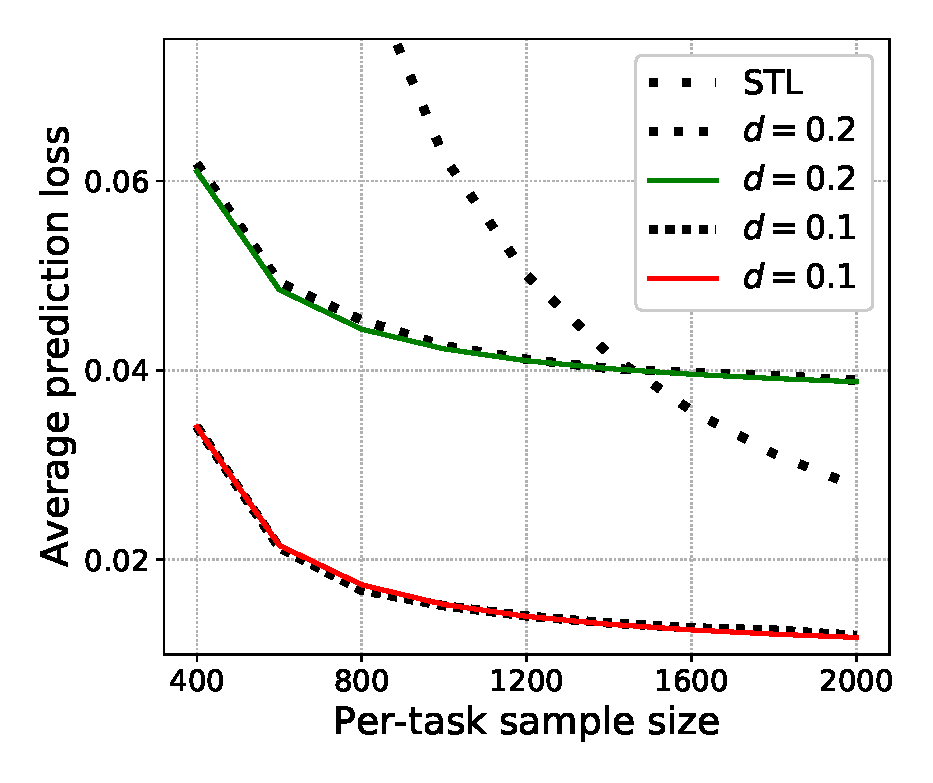
\includegraphics[width=0.9\textwidth]{figures/same_covariates.eps}
		\caption{Example \ref{ex_same_cov}}
		\label{fig_same_cov}
	\end{subfigure}\hfill
	\begin{subfigure}[b]{0.5\textwidth}
		\centering
		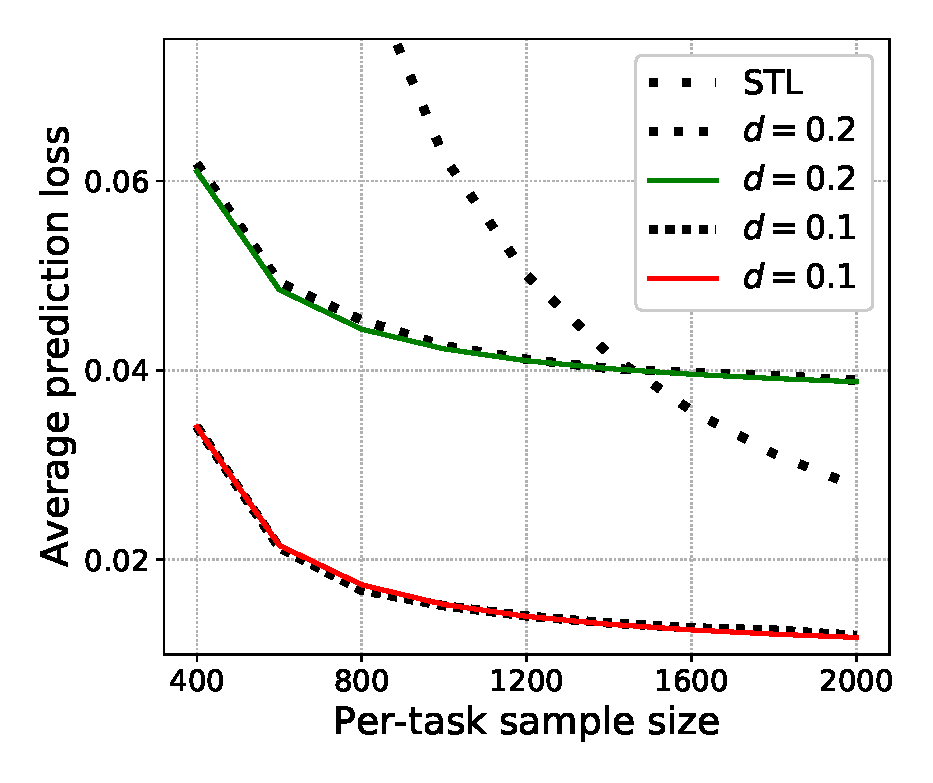
\includegraphics[width=0.9\textwidth]{figures/same_covariates.eps}
		\caption{Example \ref{ex_sample_ratio}}
		\label{fig_width}
	\end{subfigure}
%	\caption{%Three takeaways of our theory in Section \ref{sec_insight}.
%	Our estimated losses (solid line) match the empirical losses (dotted line) accurately under various settings in dimension $p = 200$.
%	\textbf{Left.} Validating Example \ref{ex_same_cov} for ten tasks: the noise variance $\sigma^2$ is $1/4$.
%	\textbf{Middle.} Validating Example \ref{ex_sample_ratio} for two tasks: we discover an interesting phenomena by fixing task two's sample size and increasing task one's sample size.
%	Moreover, our result accurately predicts the critical point (marked in circle) of the loss curve.
%	Depending on how large the distance $d^2$ is, task two's prediction loss decreases initially before increasing again, or decreases monotonically.
%	\textbf{Right.} We show how different levels of covariate shift affect hard parameter sharing when there is no bias.
%	Having covariate shift increases task two's prediction loss when task two's sample size is smaller than task one. Otherwise, having covariate shift (surprisingly) decreases task two's prediction loss.}
%	\label{fig_model_shift_phasetrans}
\end{figure*}

%Moreover, by setting $t=2$ in Theorem \ref{thm_many_tasks}, we can obtain the prediction loss for the HPS estimator for the transfer learning setting where the two tasks have the same covariates  $X^{(1)}=X^{(2)}$. For the reader's convenience, we give the precise statement in Corollary \ref{thm_two_tasks}.
%Theorem \ref{thm_many_tasks} implies Theorem \ref{thm_two_tasks} as a special case with $t=2$ and $r=1$.
%In this section, we consider the setting where the two tasks have the same covariates  $X^{(1)}=X^{(2)}$.
%We define $A^\star \in \R^{2}$ as the normalized eigenvector corresponding to the larger eigenvalue of the $2\times 2$ matrix
%$ {B^\star}^\top \Sigma  B^\star,$ where recall that $B^\star \define [{\beta}^{(1)},{\beta}^{(2)}] \in \real^{p\times 2}$ by definition.
% is the matrix formed by the linear model parameters of the two tasks.
%Without loss of generality, we assume that the two eigenvalues of ${B^\star}^\top \Sigma B^\star$ are not degenerate, so that $A^\star$ is uniquely defined. %Otherwise, Theorem \ref{thm_two_tasks} will give a null result.
%In the following corollary, the estimate \eqref{minimizer_beta1} shows that the minimizer $\hat a$ is approximately equal to $A^\star(1)/A^\star(2)$, while \eqref{Li_multi0} gives the exact asymptotic limit of $L_2(\hat{\beta}_2^{\MTL}(\hat a)) $, together with an explicit convergence rate that we believe to be sharp.

%\begin{corollary}\label{thm_two_tasks}
%Under Assumption \ref{assm_big1}, suppose that $X^{(1)}=X^{(2)}$ and $n_1=n_2\equiv n$. Let $c>0$ be an arbitrary (small) constant. Then we have that with high probability,
%\be\label{minimizer_beta1}
%\left\| u_{\hat a}u_{\hat a}^\top - A^\star {A^\star}^\top\right\|_F  \le  \left[\frac{ n^{-1/2+2/\varphi+c}  \|{B^{\star}}^{\top}\Sigma B^{\star}\|  + n^{-1/2+c} \sigma^2 }{\lambda_1 - \lambda_{2} } \right]^{1/2},
%\ee
%where $u_{\hat a}$ is the unit vector defined as
%$ u_{\hat a}:= \frac1{\hat a^2 +1} \begin{pmatrix} {\hat a}\\ %1\end{pmatrix},$ and $\lambda_1 $ and $\lambda_{2}$ are respectively the larger and smaller eigenvalues of ${B^\star}^\top\Sigma B^\star$.
%for task 2,  % over the randomness of the input,
%Moreover, the prediction loss of the HPS estimator satisfies that with high probability,
%	\begin{align}
%		& \bigabs{L_2(\hat{\beta}_2^{\MTL}(\hat a)) - \left\|(\Sigma^{(2)})^{1/2} \left(A^\star(2) \cdot B^{\star}A^{\star}  - \beta^{(2)}\right)\right\|^2  - |A^\star(2)|^2  \frac{p\sigma^2}{n-p} } \nonumber\\
%		& \le  \left[  \frac{  n^{-1/2+2/\varphi+c} \|{B^{\star}}^{\top}\Sigma B^{\star}\|+n^{-1/2+c} \sigma^2} {\lambda_1  - \lambda_2 }\right]^{1/2}   \left(\norm{\Sigma^{1/2} B^{\star}}^2+  \sigma^2\right), \label{Li_multi0}
		%\le n^{-\frac{c_{\varphi}}2} \cdot \frac{\bigbrace{ \norm{\Sigma^{1/2} B^{\star}}^2+  \sigma^2} \cdot (\bignormFro{\Sigma^{1/2} B^{\star}}^2 + \sigma^2 t)} {\lambda_r ({B^\star}^\top \Sigma B^\star)- \lambda_{r+1}({B^\star}^\top \Sigma B^\star)},
%	\end{align}
%	 where $A^\star(2)$ denotes the second entry of $A^\star$.
%	 \end{corollary}

\begin{example}[How to set the width $r$ in HPS?]
\label{ex_same_cov}
%Suppose every $\beta^{(i)}$ consists of two random components, one that is shared among all tasks and one that is task-specific.
%Thus, each task contributes a certain amount to the shared component and injects a task-specific bias.
%More precisely, %we have
An important question in applications of HPS is how to set the width $r$ of the feature layer.
We use our estimates to show that the optimal width depends on the tradeoff between the estimator's bias and variance.
Concretely, consider a random-effect model where all tasks share a model vector $\beta_0$ plus perturbations.
For every $i=1,2,\cdots, t,$, $\beta^{(i)} = \beta_0 + \wt \beta^{(i)}$, where $\wt \beta^{(i)}$ denotes the $i$-th task-specific component whose entries are i.i.d. Gaussian random variables of mean zero and variance $\frac {\kappa^2} p$.

\begin{claim}
\begin{enumerate}
	\item {\bf Positive vs. negative transfer.} The averaged HPS prediction loss is smaller than the single-task OLS prediction loss if and only if $\frac{d^2}{p}\tr \Sigma  < \frac{p\sigma^2 }{n - p}$, that is, the ``task-specific variance'' is smaller than the ``noise variance'' up to some constant factor.
	
	\item {\bf The optimal rank $r$.} If $\frac{d^2}{p}\tr \Sigma  < \frac{\sigma^2 p}{n - p}$, then the smallest averaged HPS  prediction loss is achieved when $r=1$. Hence increasing the width $r$ of the shared feature representation layer does not help.
\end{enumerate}
\end{claim}
%For our discussion below, we assume that $\kappa^2 \sim d^2 \sim \sigma^2$ and $n\sim p$. %and $d^2=\OO(\kappa^2)$.
%The more precise conditions on the relations between $d^2$, $\sigma^2$ and $\kappa^2$ are given in  \eqref{choiceofpara}.
%We assume that all the random variables have finite moments up to any order as in equation \eqref{assmAhigh2}.
\begin{proof}
    In this random-effect model, using the concentration of Gaussian random vectors (e.g. Lemma \ref{largedeviation} in the supplement  \cite{MTL_suppl}),
    %Based on the definition of the random-effect model,
    the $(i, j)$-th entry of ${B^{\star}}^{\top} \Sigma B^{\star}$ is equal to %(ignoring lower order terms)
    %\begin{align*}
    %	\beta_i^{\top} \beta_j \approx \norm{\beta_0}^2 + \frac{d^2}{2}\delta_{ij},\quad 1\le i,j \le t,
    %\end{align*}
    \begin{align}\label{betaSbeta}
    	\beta_i^{\top}\Sigma  \beta_j =\beta_0^\top \Sigma \beta_0 + \delta_{ij} \frac{d^2 }{p}\tr \Sigma + \OO\left(p^{-1/2+c}\|\beta_0\|^2+ p^{-1/2+c} d^2\right),
    \end{align}
     with high probability for any constant $c>0$. We omit the details to show the error bound using Lemma \ref{largedeviation}.
    %Note that $\norm{\beta_0}^2$ is approximately $\kappa^2$.
    With \eqref{betaSbeta}, it is easy to calculate that with high probability, the eigenvalues of ${B^{\star}}^{\top} \Sigma B^{\star}$ are given by
    $$\lambda_1=\left[1+\OO(p^{-1/2+c})\right]\cdot\left(t \beta_0^\top \Sigma \beta_0  + \frac{d^2}{ p}\tr \Sigma\right) ,$$
    and
    $$ \lambda_i=\left[1+\OO(p^{-1/2+c})\right]\cdot \frac{d^2}{ p}\tr \Sigma , \ \ i=2,\cdots, t.$$ %Therefore, by taking a rank-$1$ approximation of ${B^{\star}}^{\top} B^{\star}$, we get the average prediction loss of $B^{\star} a_i^{\star}$.
    Thus for the best rank-$r$ approximation $A^\star {A^\star}^\top$  of ${B^{\star}}^{\top}\Sigma  B^{\star}$, we have
    $$\bignorm{\Sigma^{1/2} B^{\star} (A^\star {A^\star}^{\top} - \id_{t\times t})}_F^2= [1+\OO(p^{-1/2+c})]\cdot(t-r)\frac{d^2}{ p}\tr \Sigma $$
    with high probability.
    %To see this, recall that $r$ is one and $A^{\star} {A^{\star}}^{\top}$ is the best rank-$1$ approximation of ${B^{\star}}^{\top}\Sigma B^{\star} = {B^{\star}}^{\top} B^{\star}$.
    %Hence, the above expression is equal to the sum of ${B^{\star}}^{\top} {B^{\star}}$'s bottom $t-1$ singular values.
    %In the random-effect model described above, we further assume that $\Sigma$ is isotropic as an example.
    %We show that when the rank $r$ is one, the average prediction loss of hard parameter sharing is as follows
    Then using \eqref{Li_multi2}, we obtain that
    \[ \frac{1}{t}\sum_{i=1}^t L_i(\hat{\beta}_i^{\MTL}) = \bigbrace{1 - \frac{r}{t}} \frac{d^2}{p}\tr \Sigma + \frac{r}{t} \cdot \frac{p\sigma^2 }{n - p} +\oo(\|\beta_0\|^2+d^2 + \sigma^2) ,\quad \text{w.h.p. }\]
    %We describe a proof sketch.
    %First, we show that the bias equation $L(B^{\star} a_i^{\star})$ simplifies to the following
    %\[ \frac{1}{t} \sum_{i=1}^t L(B^{\star} a_i^{\star}) = \frac{1}{t}\normFro{B^{\star} A^{\star} {A^{\star}}^{\top} - B^{\star}}^2 \approx \left(1 - \frac{1}{t}\right) {d^2}{}  . \]
    %Second, using Fact \ref{fact_tr}, one can see that the average variance is
    %\begin{align*}
    %	\frac{1}{t} \sum_{i=1}^t \sigma^2\norm{a_i^{\star}}^2 \bigtr{\Sigma (X^{\top} X)^{-1}} = \frac{\sigma^2}{t} \sum_{i=1}^t \norm{a_i^{\star}}^2 \frac{p}{n - p}
    %	= \frac{1}{t}\frac{\sigma^2 p}{n - p},
    %\end{align*}
    %because $A^{\star}$ has rank-$1$ and $\sum_{i=1}^t \norm{a_i^{\star}}^2 = 1$.
    %Combined together, we have derived the average prediction loss in the random-effect model.
    %If the error is sufficiently small, then
    %Recall that the average prediction loss of STL scales as $\sigma^2\cdot \bigtr{\Sigma (X^{\top} X)^{-1}} = \frac{\sigma^2 p}{n - p}$ by Fact \ref{fact_tr}.
    %Comparing HPS to STL, we have the following qualitative properties.
    %	Suppose $n$ is sufficiently large so that the error is negligible.
\end{proof}
\end{example}



%We demonstrate the accuracy of our results in simulations.
%While our theory is asymptotic (with error terms that are negligible when $p$ is sufficiently large), we observe that they are incredibly accurate in a moderate dimension of $p = 200$.



First, we validate the result of Example \ref{ex_same_cov}.
Figure \ref{fig_same_cov} shows the average prediction loss over ten tasks as we increase the number of samples per-task from $400$ to $2000$.
In all the parameter settings, our results estimate the empirical losses accurately.
We also observe a trend that the average prediction loss increases as we increase distance $d$ from $0.1$ to $0.2$.
Our work explains the differences between these two settings since $d^2 = 0.1^2$ is always smaller than $\frac{\sigma^2 p}{n - p}$, but $d^2 = 0.2^2$ is not.
%Second, when $d = 0.1$, we have that $d^2 \le \frac{\sigma^2 p}{n - p}$ for all values of $n$, hence the average prediction loss of hard parameter sharing is always lower than STL.
Indeed, we observe a crossover point between hard parameter sharing and STL.
Finally, for $d = 0.2$, looking horizontally, we find that HPS requires fewer samples per-task than STL to achieve the same loss level. %\FY{I do not quite understand this sentence about "3x fewer", because how much data needed depends on $d$ and the prediction loss level we are looking at. For example, at the cross point, this ratio is 1. }


%Our result from Corollary \ref{cor_MTL_loss} explains this trend.


%Covariate shift: We set $\kappa = 1$ and $d = 0$.
%We set $\rho_2 = 4$ and vary $\rho_1$ from $5$ to $25$ for sample sizes.
%We use the scale parameter $\lambda = 1$ for the curve without covariate shift and $\lambda = 2$ for the curve with covariate shift (cf. Section \ref{sec_covshift}).


%Recall that Section \ref{sec_data_size} shows that increasing the data size of the source task does not always improve the performance of MTL for the target task.
%In Figure \ref{fig_ab_data}, we show that for source task MR and target task SST, there is a transition from positive to negative transfer as we increase the data size of the source task.
%Our result provides a fine-grained insight on the covariance alignment algorithm proposed in \cite{WZR20}.
%Recall that the covariance alignment procedure in \cite{WZR20} adds an additional module between the word embedding representation and the shared module.
%When the source task data size is particularly large compared to the target task, we show that applying the covariance alignment algorithm results in more significant gains.
%In Figure \ref{fig_ab_cov}, we observe that the benefit from aligning task covariances becomes more significant for LSTM and MLP as we increase the number of datapoints of the source task.

%\begin{table}
%	\begin{center}
%		\begin{tabular}{c c c c c}
%			\toprule
%			\multirow{2}{*}{{\bf Models}} & \multicolumn{2}{c}{\begin{minipage}{1.1in}\begin{center}
%				                                                                          MR, SST, SUBJ, CR, MPQA, TREC\end{center}\end{minipage}} & \multicolumn{2}{c}{\begin{minipage}{1.1in}\begin{center}MR, SST, SUBJ, CR, MPQA\end{center}\end{minipage}} \\
%			\cmidrule(lr){2-3} \cmidrule(lr){4-5}
%			& {\bf Stanford} & {\bf Alignment} & {\bf Stanford} & {\bf Alignment} \\
%			\midrule
%			{\bf MLP}  & > 100\% & 39\% & 25\% & 25\% \\
%			{\bf LSTM} & 36\% & 36\% & 28\% & 25\% \\
			% {\bf CNN}  & 76\% & - & 32\% & -\\
%			\bottomrule
%		\end{tabular}
%	\end{center}
%	\caption{Taskonomy experiment.}
%	\label{tab:taskonomy}
%\end{table}
%\begin{figure}[!t]
%	\centering
%	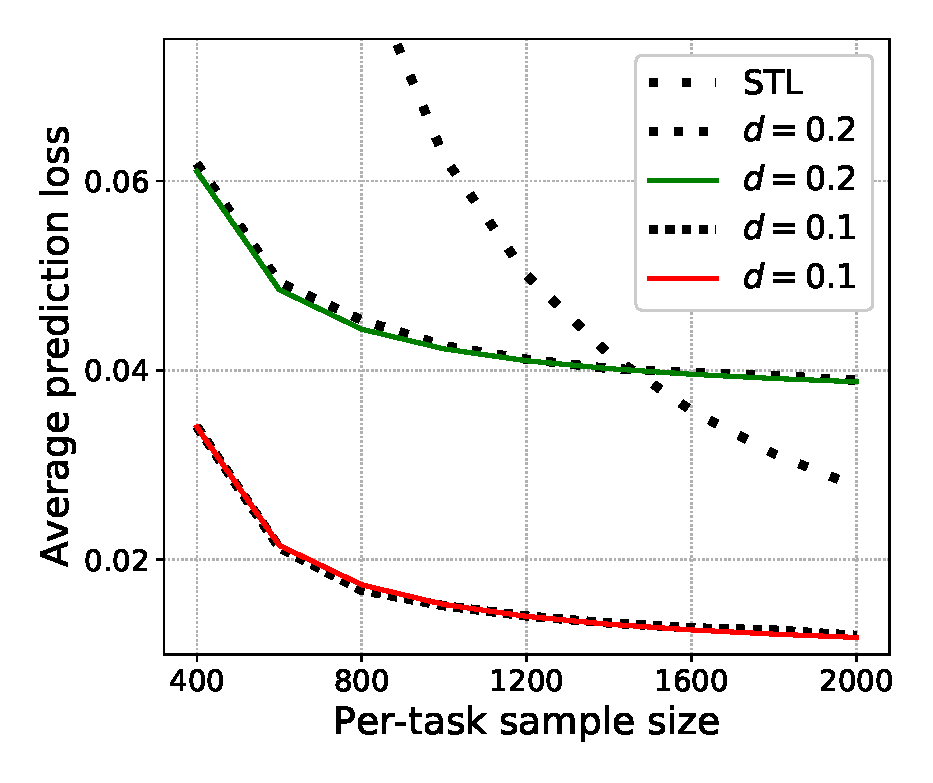
\includegraphics[width=0.35\textwidth]{figures/same_covariates.eps}
%	\caption{Validating Example \ref{ex_same_cov} in Section \ref{sec_same} for $10$ tasks: our estimated loss (solid line) matches the empirical loss (dotted line) accurately for various task-specific variance $d^2$ and sample size $n$ settings. The feature dimension $p$ is $200$, and noise variance $\sigma^2$ is $1/4$.}
%	\label{fig_same_cov}
%\end{figure}





%The estimate \eqref{minimizer_beta1} shows that the minimizer $\hat a$ is approximately equal to $A^\star(1)/A^\star(2)$, while \eqref{Li_multi0} gives the exact asymptotic limit of $L_2(\hat{\beta}_2^{\MTL}(\hat a)) $, together with an explicit convergence rate that we believe to be sharp.


%It is not hard to extend the above result to the cases with more than two tasks. We make this extension for the following reasons. First, it provides a clearer geometric intuition than the two-task setting as we will discuss below. Second, the corresponding multi-task setting is prevalent in applications of multi-task learning to image classification, where there are multiple prediction labels/tasks for every image \cite{chexnet17,EA20}. Finally, it provides useful insights into a more general theory of multi-task learning, which we will explore in greater details in future works.

%We consider an arbitrary local minimum $B, W_1, \dots, W_2$ of the optimization objective.
%We extend the bias-variance decomposition from the two-task case to the multiple-task case.
%We observe that the expected prediction loss of $\hat{\beta}_t^{\MTL}$ conditional on $X$ consists of a bias and a variance equation as follows
%\begin{align}
%	\exarg{\varepsilon_1, \dots, \varepsilon_t}{L(\hat{\beta}_t^{\MTL}) \mid X}
%	=& \bignorm{\Sigma^{1/2} \bigbrace{B^{\star} \cW^{\top} (\cW \cW^{\top})^{-1} W_t - \beta_t}}^2 \label{eq_bias_multiple} \\
%	&+ \sigma^2 \cdot (W_t^{\top} (\cW \cW^{\top})^{-1} W_t) \cdot \bigtr{\Sigma (X^{\top} X)^{-1}} \label{eq_var_multiple}
%\end{align}
%One can see that equation \eqref{eq_bias_multiple} is the bias of the multi-task learning estimator and equation \eqref{eq_var_multiple} is its variance.
%Compared to the prediction loss of single-task learning (cf. equation \eqref{eq_var_stl}), we observe that the variance equation \eqref{eq_var_multiple} is always smaller because $W_t^{\top} (\cW \cW^{\top})^{-1} W_t \le 1$.
%On the other hand, the bias equation \eqref{eq_bias_multiple} is always larger because of the difference between the task models.
%We show the generalization error of hard parameter sharing estimators.
%Before stating the result, we define the following notations.




%The key step for proving Theorem \ref{thm_many_tasks} is a characterization of $f(A, B)$'s global minimizer.
%\medskip
%
%\noindent\textbf{Comparison to single-task learning (STL).}
%Theorem \ref{thm_many_tasks} provides a sharp generalization error bound that is asymptotically tight when $n$ goes to infinity.
%%The limiting loss of hard parameter sharing consists of two parts, a bias term $L(B^{\star} a_i^{\star})$ that measures the error of $B^{\star} a_i^{\star}$, and a variance term that scales with noise variance $\sigma^2$.
%%	Our result implies that the variance of hard parameter sharing is always smaller than single-task learning.
%%	This is because	STL's variance is equal to $\frac{\sigma^2 \cdot p} {n - p}$ by Fact \ref{lem_minv}, and $\norm{a_i^{\star}}^2 \le 1$ since the spectral norm of $U_r$, which is a projection matrix, is at most one.
%One direct implication of our result is that compared to STL, the variance always decreases, since STL's variance is equal to $\sigma^2 \tr[\Sigma (X^{\top} X)^{-1}]$.
%On the other hand, the bias always increases.


%\FY{add simulations to check our results; discuss motivations and possible applications}
\iffalse
In this paper, we consider a natural extension of the estimator $\hat \beta^{\rm{TL}} $, that is, the \emph{hard parameter sharing} (HPS) estimator, which has been a standard type of estimator in multi-task learning \FY{citations}. More precisely, we study the following HPS architecture: a shared feature representation layer $B\in\real^{p}$ for all datasets and a separate output layer $A_i \in \real$ for every dataset $i$. Then we study the following minimization problem:
\begin{align}\label{eq_tsl}
			f(A, B) = \norm{X^{(1)} B A_1 - Y^{(1)}}^2 + \norm{X^{(2)} B A_2 - Y^{(2)}}^2,
\end{align}
where we abbreviate $A = [A_1, A_2]$. Let $(\hat{A}, \hat{B})$ be the minimizer of $f(A, B)$. We define the hard parameter sharing (HPS) estimator for task $i$ as
\be\label{def_HPS}\hat{\beta}_i^{\MTL} = \hat{B} \hat{A}_i,\quad i=1,2.\ee
Note that $\hat \beta^{\rm{TL}}$ is a special case of $\hat{\beta}_i^{\MTL}$ by setting $A_1=A_2=1$.

For the optimization objective $f(A, B)$ in \eqref{eq_tsl}, using the local optimality condition $\frac{\partial f}{\partial B} = 0$, we can solve that
	\begin{align}
		\hat{B} = A_2^{-1} \hat \Sigma(a)^{-1} \left[a (X^{(1))})^{\top}Y^{(1)} +  (X^{(2)})^{\top}Y^{(2)}\right], \label{eq_Bhat_2task} %\\
		%&= (B^\star A ^{\top}) (A A^{\top})^{-1} + (X^{\top}X)^{-1}X^{\top}   \bigbrace{\sum_{j=1}^t \varepsilon_i A_i^{\top}} (A  A^{\top})^{-1}.
	\end{align}
where we denote $a:=A_1/A_2$ and $\hat \Sigma(a):= a^2 (X^{(1)})^\top X^{(1)}  + (X^{(2)})^\top X^{(2)}$.
Applying $\hat B$ to equation \eqref{eq_tsl}, we obtain an objective that only depends on $a $ as follows %\HZ{$A$ has been used to denote the output layers. Could you replace $A$ with another symbol (say $x$)?}
 \begin{align}
		 g(a) \define & \left\| X^{(1)} \hat\Sigma(a)^{-1} (X^{(2)})^\top X^{(2)} (a\beta^{(2)}-\beta^{(1)}) \right. \nonumber\\
			& \left. + \left(a^2 X^{(1)}\hat \Sigma(a)^{-1} (X^{(1)})^\top-\id_{n_1\times n_1}\right)\epsilon^{(1)}+ a X^{(1)}\hat \Sigma(a)^{-1} (X^{(2)})^\top \epsilon^{(2)} \right\|^2 \nonumber\\
		   +& \left\| X^{(2)} \hat \Sigma(a)^{-1} (X^{(1)})^\top X^{(1)} (a\beta^{(1)}-a^2\beta^{(2)}) \right. \nonumber\\
		  &\left.+ \left(X^{(2)}\hat\Sigma(a)^{-1} (X^{(2)})^\top-\id_{n_2\times n_2}\right)\epsilon^{(2)} + a X^{(2)}\hat \Sigma(a)^{-1} (X^{(1)})^\top \epsilon^{(1)} \right\|^2. \label{eq_mtl_A12}
	\end{align}
Let $\hat a$ be the minimizer of $g(a)$. Throughout this paper, we regard $Y^{(1)}$ as the source data, and $Y^{(2)}$ as the target data.  Then the HPS estimator \eqref{def_HPS} for the target task 2 is
\be\label{HPS_est}
\hat{\beta}_2^{\MTL} (\hat a) = \hat \Sigma(\hat a)^{-1}  \left[\hat a (X^{(1))})^{\top}Y^{(1)} +  (X^{(2)})^{\top}Y^{(2)}\right].
\ee
\fi

